%! Author = user
%! Date = 22.06.2022

% Preamble
\documentclass[11pt]{article}

% Packages
%----------------------------------------------------------------------------------------
%	PACKAGES AND OTHER DOCUMENT CONFIGURATIONS
%----------------------------------------------------------------------------------------

\usepackage{listings}
\usepackage{graphicx}
\usepackage{booktabs}
\usepackage{enumitem}
\usepackage[left=2cm,right=2cm,
    top=2cm,bottom=2cm,bindingoffset=0cm]{geometry}
\usepackage[utf8]{inputenc}
\usepackage[english,russian]{babel}
\usepackage{titling}
\usepackage{textcomp}
\usepackage{mathtext}
\usepackage{amsmath,amsfonts,amssymb,amsthm,mathtools}
\usepackage{icomma}
\usepackage{import}
\usepackage{amssymb, amsmath}
\usepackage{indentfirst}
\usepackage{moresize}
\usepackage{multicol}
\usepackage{dsfont}
\usepackage{xifthen}
\usepackage{pdfpages}
\usepackage{transparent}
\usepackage{caption}
\usepackage{epigraph}
\usepackage{xcolor}

\newtheorem{statement}{Statement}
\newtheorem{corollary}{Corollary}
\newtheorem{theorem}{Theorem}
\newtheorem{definition}{Definition}
\newtheorem{lemma}{Lemma}
\newtheorem{example}{Example}
\theoremstyle{remark}
\newtheorem{remark}{Remark}
\newtheorem{prop}{Property}




\numberwithin{equation}{section} % Number equations within sections (i.e. 1.1, 1.2, 2.1, 2.2 instead of 1, 2, 3, 4)
\numberwithin{figure}{section} % Number figures within sections (i.e. 1.1, 1.2, 2.1, 2.2 instead of 1, 2, 3, 4)
\numberwithin{table}{section} % Number tables within sections (i.e. 1.1, 1.2, 2.1, 2.2 instead of 1, 2, 3, 4)

\setlength\parindent{0pt} % Removes all indentation from paragraphs

\setlist{noitemsep} % No spacing between list items

%%% Операторы всякие:
\DeclareMathOperator{\arsec}{arsec}
\DeclareMathOperator{\arcsch}{arcsch}
\DeclareMathOperator{\arcosh}{arcosh}
\DeclareMathOperator{\arsinh}{arsinh}
\DeclareMathOperator{\artanh}{artanh}
\DeclareMathOperator{\arsech}{arsech}
\DeclareMathOperator{\grad}{grad}
\DeclareMathOperator{\Log}{Log}
\DeclareMathOperator{\Arg}{Arg}
\renewcommand{\Im}{\mathop{\mathrm{Im}}\nolimits}
\renewcommand{\Re}{\mathop{\mathrm{Re}}\nolimits}
\DeclareMathOperator{\arcoth}{arcoth}
\usepackage{setspace}
%%% Колонтитулы
\usepackage{fancyhdr}
\pagestyle{fancy}
\renewcommand{\sectionmark}[1]{\markright{\thesection\ #1}}

\fancyhead[LE,RO]{\thepage}
\fancyhead[LO]{\rightmark}
\fancyhead[RE]{\leftmark}


%----------------------------------------------------------------------------------------
%	SECTION TITLES
%----------------------------------------------------------------------------------------

%\sectionfont{\vspace{6pt}\centering\normalfont\scshape} % \section{} styling
%\subsectionfont{\normalfont\bfseries} % \subsection{} styling
%\subsubsectionfont{\normalfont\itshape} % \subsubsection{} styling
%\paragraphfont{\normalfont\scshape} % \paragraph{} styling

\newcommand{\RNumb}[1]{\uppercase\expandafter{\romannumeral #1\relax}}

\renewcommand\thesection{\arabic{section}.}
\renewcommand\thesubsection{\thesection\arabic{subsection}}
\renewcommand\thesubsubsection{\thesubsection.\arabic{subsubsection}}
\renewcommand{\bf}{\textbf}
%----------------------------------------------------------------------------------------
%	HEADERS AND FOOTERS
%----------------------------------------------------------------------------------------
\DeclareMathOperator{\ord}{ord}
\DeclareMathOperator{\ld}{ld}
\DeclareMathOperator{\exi}{exi}
\DeclareMathOperator{\num}{num}
\DeclareMathOperator{\den}{den}
\DeclareMathOperator{\diam}{diam}
\DeclareMathOperator{\sign}{sign}
\DeclareMathOperator{\len}{len}
\DeclareMathOperator{\vp}{v.p.}
\DeclareMathOperator{\osc}{osc}
\newcommand{\divisible}{\mathop{\raisebox{-2pt}{\vdots}}}
\DeclareRobustCommand{\divby}{%
     \mathrel{\text{\vbox{\baselineskip.65ex\lineskiplimit0pt\hbox{.}\hbox{.}\hbox{.}}}}%
}
\newcommand{\eqdef}{\stackrel{\mathrm{def}}{=}}
\DeclareRobustCommand{\notdivby}{%
     \!\!\not\;\divby%
}
\DeclareMathOperator{\Int}{Int}
\DeclareMathOperator{\Cl}{Cl}
\DeclareMathOperator{\Fr}{Fr}
\newcommand{\Mod}[1]{\ (\mathrm{mod}\ #1)}



\addto{\captionsrussian}{\renewcommand{\abstractname}{АННОТАЦИЯ}}

\newcommand{\incfig}[1]{%
    \def\svgscale{1.5}
    \import{./figures/}{#1.pdf_tex}
}
\graphicspath{{pictures/}}
\DeclareGraphicsExtensions{.pdf,.png,.jpg, .jpeg, .tex}

\definecolor{myblue}{RGB}{72, 184, 178}
\definecolor{myblue1}{RGB}{0, 109, 167}
\usepackage{color}
\usepackage[colorlinks,urlcolor = blue, filecolor=blue,citecolor=blue, linkcolor = blue]{hyperref}

% Document
\begin{document}
    \begin{titlepage}
	\centering
	
	{\Large \textsf{Летняя математическая школа ЛНМО} \par}
	
	\vspace{0.3cm}
	
	{\large \textsf{Поставы, 2022г.}\par}
	
	\vspace{1 cm}
	
	{\HUGE \textsf{Алгебраическая геометрия \\ и теория чисел} \par}
	
	\vspace{0.5cm}
	
	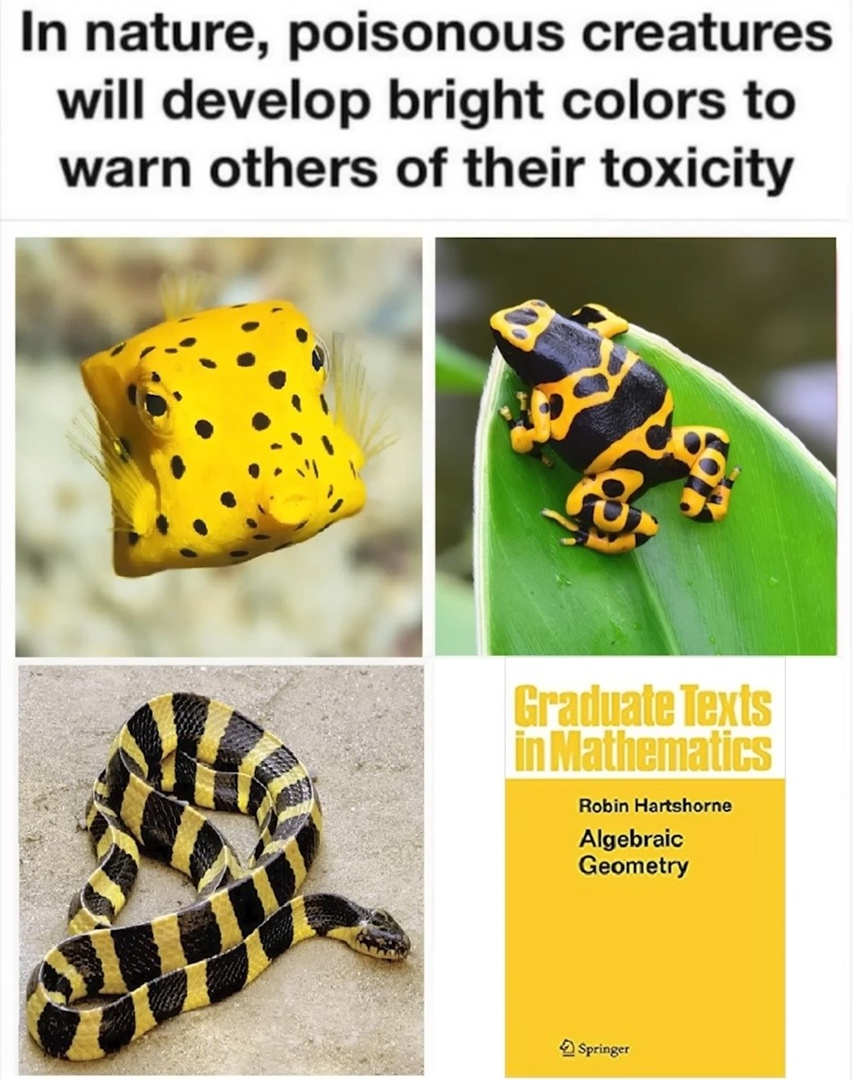
\includegraphics[scale = 0.4]{Title.jpg}
	
	\vspace{0.2cm}
	
	{\large \textsf{\textit{Конспект по материалам лекций, прочитанных М.И. Магиным \\ 11-му математическому классу}} \par}
	\vfill
	
	\begin{minipage}{6in}
		\centering
		\raisebox{-0.5\height}{
\includegraphics[width=0.46\textwidth]{lnmo logo}}
	\end{minipage}


\end{titlepage}

    \begin{center}
        \section*{Алгебраическая геометрия и теория чисел}
    \end{center}
    \tableofcontents
    \newpage

    \section{Нормированные поля}
    \subsection{Нормированное поле. Неархимедовы нормы.}
    Здесь и в дальнейшем будем полагать $F$ полем, хотя многие вещи работают и для кольца (а для области целостности существует
    единственное продолжение на поле частных).

    \begin{definition}\label{fieldnorm}
     Нормой (нормированием, абсолютным значением) на поле $F$  называют отображение $\| \cdot \|\colon F \to \mathbb{R}_{> 0}$,
        удовлетворяющее следующим свойствам:
        \begin{enumerate}
            \item $\| x \| = 0 \Leftrightarrow x = 0$.

            \item $\forall x, y \in F \ \| x y \| = \| x \| \| y \| $.

            \item $\exists C > 0\colon \forall x, y \in F\colon$
            \[ \| x + y \| \le C \cdot \max(\| x \|, \| y \| ). \]
        \end{enumerate}
        Пара $(F, \| \cdot \|)$ называется нормированным полем.
    \end{definition}
    \begin{remark}
        Тем, кто уже до этого видел определение нормы, это определение может показаться странным, так как обычно вместо третьего свойства
        требуют неравенство треугольника:
        \[ \forall x, y \in F \ \| x + y \| \le \| x \| + \| y \| \]
        Ясно, что третье свойство следует из неравенства треугольника с $C = 2$. Ниже мы покажем и обратную импликацию.
    \end{remark}

    Ясно, что любая норма задаёт метрику $d(x, y) = \| x - y \|$, а любая метрика индуцирует топологию стандартным образом.

    \begin{example}
        Если $F \le \mathbb{C}$, то подходит $| \cdot |$ (модуль комплексного числа). Если $F \le \mathbb{R}$ или $F \le \mathbb{Q}$, то подходит $| \cdot |$.
    \end{example}

    \begin{example}
        На любом поле можно ввести тривиальную норму (иногда соответствующую ей метрику называют метрикой лентяя):
        \[ \| x \| = \begin{cases} 0, x = 0 \\ 1, x \neq 0 \end{cases}\]
    \end{example}

    \begin{theorem}
        Если в определении \ref{fieldnorm} постоянная $C$ равна $2$, то норма удовлетворяет неравенству треугольника.
    \end{theorem}
    \begin{proof}

        Сначала отметим, что если $n, m \in \mathbb{N}, \ n \le 2^m$, то в случае произвольной постоянной $C$ выполняется оценка:
        \[ \| x_1 + x_2 + \ldots  + x_n \| \le C^m \cdot \| \max\limits_{1 \le k \le n} \| x_k \| \]
        В самом деле, достаточно просто расписать дерево неравенств. \\
        Отсюда следует неравенство
        \[ \| x_1 + \ldots + x_n \| \le (2n)^{c_0} \max\limits_{1 \le k \le n}(\| x_k \|), \quad c_0 = \log_2{C} \]
        В самом деле, $(2n)^{\log_2{C}} = C \cdot n^{\log_2{C}}$.
        Это также даёт удобную оценку: $\| n \| \le (2n)^{c_0}$.\\
        Теперь заметим, что в нашем случае $c_0 = \log_2{C} = \log_2{2} = 1$, а значит, мы можем провести вот такую
        оценку:
        \begin{multline*} \| x + y \|^n = \| (x + y)^n \| = \left\| \sum\limits_{k = 0}^{n} \binom{n}{k} x^k y^{n - k} \right\| \le 2(n + 1) \max\limits_{0 \le k \le n}\left\| \binom{n}{k} x^k y^{n - k} \right\| \le 2(n + 1) \max\limits_{0 \le k \le n}\left( 2 \binom{n}{k} \|x\|^k \| y \|^{n - k} \right) \le \\
        \le 4(n + 1) (\| x \| + \| y \| )^n \end{multline*}
        Преобразуем это неравенство
        \[ \left( \frac{\| x + y \| }{\| x \| + \| y \|} \right)^n \le 4(n + 1) \Leftrightarrow  \frac{\| x + y \|}{\| x \| + \| y \| } \le 4^{\frac{1}{n}} \cdot (n + 1)^{\frac{1}{n}} \]
        В пределе при $n \to \infty$ получаем:
        \[ \frac{\| x + y \| }{\| x \| + \| y \| } \le 1 \Leftrightarrow \| x + y \| \le \| x \| + \| y \| \]
    \end{proof}

    \begin{remark}
        Пример $F = \mathbb{C}$ с нормой $\| \cdot \| = | \cdot |^{\alpha}, \ \alpha > 1$ показывает, что константу $C = 2$ нельзя улучшить.
    \end{remark}
    \begin{corollary}
        Норма непрерывна.
    \end{corollary}
    \begin{definition}
        Нормы, с постойнной $C = 1$ в определении \ref{fieldnorm} называют неархимедовыми. Нормы, не являющиеся неархимедовыми,
        называют архимедовыми.
    \end{definition}
    \begin{example}
        Тривиальная норма на любом поле $F$ является неархимедовой.
    \end{example}
    \begin{definition}
        Ясно, что любое $x \in \mathbb{Q}$ представимо в виде $x = p^n \cdot \frac{a}{b}$, где $a, b \in \mathbb{Z}, \ a \not\divisible p$, $b \not\divisible p, \ \gcd(a, b) = 1$, а $n \in \mathbb{Z}$.
        В таком случае число $n$ называют $p$-адическим показателем числа $x$ и обозначают $\upsilon_p(x)$.
    \end{definition}
    \begin{definition} \textbf{(Самое важное)}\\
    Пусть $p$~--- простое число. Тогда норму
        \[ \| x \|_{p} = \begin{cases} 0, x = 0 \\ p^{-\upsilon_p(x)}, x \neq 0  \end{cases}\]
    на поле $\mathbb{Q}$ называют $p$-адической нормой.
    \end{definition}

    \begin{remark}
        Ясно, что подоходит $r^{-\upsilon_p(x)}$, где $r > 1$, но $p$ брать удобно, так как для $x \in \mathbb{Q}^{*}$ справедлива формула произведения
        \[ 1 = \prod\limits_{p} |x| \cdot  \| x \|_{p} \]
    \end{remark}
    \begin{lemma}
        Если норма неархимедова, то для $x, y\colon \| x \| \neq \| y \|$ выполняется $\| x + y \| = \max\{\| x \|, \| y \| \}$.
    \end{lemma}
    \begin{corollary}
        Рассмотрим $(F, \| \cdot \| )$, где норма $\| \cdot \|$ неархимедова. Тогда, если  $b \in B_r(a)$, то $B_r(a) = B_r(b)$.
     \end{corollary}
    \begin{corollary} (Забавное)\\
        Если на поле $F$ введена неархимедова норма $F$, то $\forall x, y, z \in F$ по крайней мере два числа из
        $\| x - y \|, \ \| x - z \|, \ \| y - z\| $ равны. \\
        Иными словами, в метрическом пространстве $(F, d)$ ($d(x, y) = \| x - y \| $) все треугольники равнобедренные.
    \end{corollary}

   \section{$p$-адические числа}
   \subsection{Кольцо целых $p$-адических чисел.}

    Прежде чем давать какие-либо определения, рассмотрим следующий мотивирующий пример. \\
    Рассмотрим сравнение $x^2 \equiv 2 \pmod{7^n}$, $n \in \mathbb{N}$. Если $n = 1$, то ясно, что
    \[ x_0 \equiv \pm 3 \pmod{7} \]
    Теперь рассмотрим $n = 2$. $x^2 \equiv 2 \pmod{7^2} \Rightarrow x^2 \equiv 2
    \pmod{7}$, а значит, решения сравнения с $n = 2$ надо искать в виде $x_0 + 7t_1$.\\
    Займемся поиском решений вида $x_1 = 3 + 7t_1$. Подставим:
    \[ (3 + 7t_1)^2 \equiv 2 \pmod{7^2} \Leftrightarrow 9 + 6 \cdot 7t_1 + 7^2 t_1^2 \equiv 2 \pmod{7^2} \Rightarrow 1 + 6t_1 \equiv 0 \pmod{7} \Rightarrow t_1 \equiv 1 \pmod 7 \]
    Отсюда имеем решение  $x_1 \equiv 3 + 7 \cdot 1 \pmod{7^2}$.\\
    При $n = 3$ мы получим $x_2 = x_1 + 7^2 t_2$, и, подставляя
    \[ (3 + 7 + 7^2 t_2)^2 \equiv 2 \pmod{7^3}, \]
    мы найдём $t_2 \equiv 2 \pmod{7}$, а значит,
    \[ x_2 \equiv 3 + 7 \cdot 1 + 7^2 \cdot 2 \pmod{7^3} \]
    Продолжая этот процесс, получим последовательность $x_0, x_1, x_2, \ldots, x_n, \ldots$ со свойствами
    \[ x_0 \equiv 3 \pmod{7}, \quad x_n \equiv x_{n - 1} \pmod{7^n}, \quad x_n^2 \equiv \pmod{7^{n + 1}} \]

    Процесс построения этой последовательности может напонмить внимательному читателю процесс вычисления $\sqrt{2}$
    при помощи приближения рациональными числами. Там мы тоже строим последовательность рациональных чисел
    $r_1, r_2, \ldots, r_n$, квадраты которых становятся сколь угодно близки к 2, например, $|r_n^2 - 2|< 1/10^n$.

    Если мы зафиксируем простое число $p$, будем считать два целых числа близкими, если их разность делится на достаточно большую
    степень $p$ (то есть, близкими в смысле $p$-адической метрики):
    \[ d_p(x, y) = \| x - y \|_p = p^{-\upsilon_p(x - y)}\]
    В конкретном примере выше,
    \[ \forall \varepsilon > 0 \ \exists N\colon \forall n \ge N \  d_7(x_n^2, 2) < \varepsilon \]
    Как мы помним, задание последовательности рациональных чисел $\{ r_n \}$ определяет вещественное число $\sqrt{2}$.
    Проводя аналогию, здесь мы также можем предположить, что последовательность $\{ x_n \}$ определяет некоторое
    число $\alpha$ совершенно новой природы. \\
    Заметим также, что если у нас есть такая последовательность рациональных чисел $\{ r'_n \}$, что \\$\forall \varepsilon > 0 \ \eists N\colon \forall n > N \ |r_n - r'_n| < \varepsilon $, то
    её пределом также будет $\sqrt{2}$ (и в этом смысле определение корректно).\\
    Соответсвенно, здесь нам также будет естественно предположить, что последовательность $\{ x'_n \}$, для которой $x_n \equiv x'_n \pmod{7^{n + 1}}$, определяет то же самое число $\alpha$.
    \begin{remark}
        В общем, во всей этой аналогии мы просто заменили метрику на $p$-адическую.
    \end{remark}
    \begin{definition}
        Пусть $p$~--- некоторое простое число. Последовательность целых чисел $\{ x_n \}$, обладающих свойством
        \[ x_n \equiv x_{n - 1} \pmod{p^n} \ \forall n \ge 1\]
        определяет новый объект, называемый $p$-адическим числом. Две последовательности $\{ x_n \}$ и $\{ x'_n \}$ определяют одно и то же
        целое $p$-адическое число, когда $x_n \equiv x'_n \pmod{p^{n + 1}} \ \forall n \ge 0$.\\
        То есть, целые $p$-адические числа~--- предел по $p$-адическое норме целых.\\
        Множество всех целых $p$-адических чисел мы будем обозначать через $\mathbb{Z}_p$.\\
    \end{definition}
    Обычные целые числа (не $p$-адические) будем с этого момента называть целыми рациональными.\\


    Заметим, что каждому целому рациональному числу $x$ можно сопоставить целое $p$-адическое число, определяемое последовательностью
    $\{ x, x, x, \ldots \}$. Такое целое $p$-адическое число мы будем обозачать той же буквой $x$. Таким образом, мы получили естественное
    вложение $\mathbb{Z} \hookrightarrow \mathbb{Z}_p$ (инективность вполне очевидна).

    \begin{remark} \textbf{Канонический способ задания $p$-адического числа.}\\
        Пусть целое $p$-адическое число задается последовательностью $\{ x_n \}$. Обозначим наименьшее неотрицательное
        число, сравнимое с $x_n$ по модулю $p^{n + 1}$ за $\overline{x_n}$.
        \[ x_n \equiv \overline{x_n} \pmod{p^{n + 1}}, \ 0 \le \overline{x_n} < p^{n + 1} \]
        Ясно, что
        \[ \overline{x_n} \equiv x_n \equiv x_{n - 1} \equiv \overline{x_{n - 1}} \pmod{p^n}\]
        То есть, последовательность $\{ \overline{x_n} \}$ определяют то же целое $p$-адическое число, что и $\{ x_n \}$.
        Заметим, что если две последовательности $\{ \overline{x_n} \}$ и $\overline{y_n}$ определяют одно и то же целое $p$-адическое число, то
        в силу
        \[ \overline{x_n} \equiv \overline{y_n} \pmod{p^{n + 1}}, \ 0 \le \overline{x_n} < p^{n + 1}, \ 0 \le \overline{y_n} < p^{n + 1}\]
        мы имеем $\overline{x_n} = \overline{y_n}$, то есть, такое представление единственно. Его мы и будем называть каноническим представлением. \\


        Заметим, что $\overline{x^n} \equiv \overline{x_{n - 1}} \pmod{p^n}$, а так как $0 \le \overline{x_n} < p^{n + 1}$, вся каноническая
        последовательность имеет вид
        \[ \{ a_0, \ a_0 + a_1 p, \ a_0 + a_1 p + a_2 p^2, \ldots \}, \quad 0 \le a_i < p \]
        С другой стороны, ясно, что каждая последовательность такого вида задаёт некоторое целое $p$-адическое число.
    \end{remark}

    Ясно, что операции сложения и умножения на $p$-адических числах определяются поточечными операциями с соответствующими
    последовательностями.

    Все свойства операций очевидны, значит, $\mathbb{Z}_p$~--- коммутативное кольцо. Поймём что-нибудь про множество обратимых элементов кольца.

    \begin{theorem} \label{UnitP-adic}
        Целое $p$-адическое число $\alpha$, определяемое
        последовательностью $\{ x_0, x_1, \ldots, x_n, \ldots \}$ обратимо тогда и только тогда, когда $x_0 \not\equiv 0 \pmod{p}$.
    \end{theorem}
    \begin{proof}
        Путь $\alpha \in \mathbb{Z}_p^{*}$. Тогда существует такое целое $p$-адическое число $\beta$, что $\alpha \beta = 1$. \\
        Пусть $\beta$ определяется последовательностью $\{ y_n \}$. Тогда
        \[ x_n y_n \equiv 1 \pmod{p^{n + 1}} \]
        В частности, $x_0 y_0 \equiv 1 \pmod{p} \Rightarrow x_0 \not\equiv 0 \pmod{p}$. И обратно, так как $x_0 \not\equiv 0 \pmod{p}$ и $x_n \equiv x_{n - 1} \pmod{p^n}$ мы имеем
        \[ x_n \equiv x_{n - 1} \equiv \ldots \equiv x_0 \pmod{p} \Rightarrow x_n \not\equiv 0 \pmod{p} \]
        Значит, так как $p$~--- простое, $\forall n \ \exists y_n \colon x_n y_n \equiv 1 \pmod{p^{n + 1}}$.
        \[ x_n \equiv x_{n - 1} \pmod{p^n}, \ x_n y_n \equiv x_{n - 1} y_{n - 1} \pmod{p^n} \Rightarrow y_n \equiv y_{n - 1} \pmod{p^n} \]
        а значит, $\{ y_n \}$ определяет некоторое целое $p$-адическое число $\beta$.\\
        Таким образом, $\alpha \beta = 1 \Rightarrow \alpha \in \mathbb{Z}_p^{*}$.
    \end{proof}

    \begin{theorem}\label{predstp-adic}
        Любое отлчиное от нуля целое $p$-адическое число $\alpha$ можно единственным образом представить в виде
        \[ \alpha = p^m \cdot \varepsilon, \quad \varepsilon \in \mathbb{Z}_p^{*}, \ m \in \mathbb{N} \]

    \end{theorem}
    \begin{proof}
        Если $\alpha \in \mathbb{Z}_p^{*}$, то равенство справедливо при $m = 0$.\\
        Пусть теперь $\alpha \notin \mathbb{Z}_p^{*}$ и $\{ x_n \} \to \alpha$. Тогда, по предыдущей теореме
        $x_0 \equiv 0 \pmod{p}$. Так как $\alpha \neq 0, \ \exists N \in \mathbb{N}\colon \forall n \ge N \ x_n \not\equiv 0 \pmod{p^{n + 1}}$.
        Пусть $m$~--- наимеьший индекс, для которого
        \[ x_m \not\equiv 0 \pmod{p^{m + 1}}\]
        Заметим, что в таком случае $\forall s \ge 0$
        \[ x_{m + s} \equiv x_{m - 1} \equiv 0 \pmod{p^{m}} \Rightarrow y_s = \frac{x_{m + s}}{p^m} \in \mathbb{Z} \]
        \[ p^m y_s - p^m y_{s - 1}  = x_{m + s} - x_{m + s - 1} \equiv 0 \pmod{p^{m + s}} \Rightarrow y_s \equiv y_{s - 1} \pmod{p^s}\]
        То есть, последовательность $\{ y_s \}$ тоже определяет некоторое $p$-адическое число $\varepsilon \in \mathbb{Z}_p$.
        Заметим, что $y_0 = x_m/p^m \not\equiv 0 \pmod{p} \Rightarrow \varepsilon \in \mathbb{Z}_p^{*}$.\\
        Из сравнения
        \[ p^m y_s = x_{m + s} \equiv x_s \pmod{p^{s + 1}} \]
        следует, что $\alpha = p^m \cdot \varepsilon$.
        Покажем теперь единственность. Предположим, что $\alpha = p^k \xi, \ k \ge 0, \ \xi \in \mathbb{Z}_{p}^{*}$. Пусть $\{ z_s \} \to \xi$.
        \[ p^m y_s \equiv p^k z_s \pmod{p^{s + 1}} \ \forall s \ge 0 \]
        Так как $\varepsilon$ и $\xi$~--- обратимые элементы кольца, по предыдущей теореме $y_s \not\equiv 0 \pmod{p}, \ z_s \not\equiv 0 \pmod{p}$.
        Подставим в предыдущее сравнения $s = m$:
        \[ p^m y_m \equiv p^k z_m \not\equiv 0 \pmod{p^{m + 1}} \Rightarrow k \le m \]
        Так как мы можем проделать то же самое абсолютно симметрично для $k$, мы также имеем $k \ge m$, а значит
        $k = m$.
        То есть, мы получили, что $y_{m + s} \equiv z_{m + s} \pmod{p^{s + 1}}$, а так как $y_{s + 1} \equiv y_s \pmod{p^{s + 1}}, \ z_{s + 1} \equiv z_s \pmod{p^{s + 1}}$,
        мы имеем $z_s \equiv y_s \pmod{p^{s + 1}} \ \forall s \ge 0 \Rightarrow \varepsilon = \xi$.
    \end{proof}
    \begin{corollary}
        $\mathbb{Z}_p$~--- область целостности.
     \end{corollary}
    \begin{proof}
        Упражнение в листочке.
    \end{proof}

    Теперь ясно, что число $m$ в представлении $\alpha = p^m \varepsilon$~--- $p$-адический показатель $\alpha$ ($\upsilon_p(\alpha)$).

    В терминах $p$-адического показателя легко вырадать свойства делимости $p$-адических чисел.
    \begin{corollary}
        Целое $p$-адическое число $\alpha$ делится на целое $p$-адическое число $\beta$ тогда и только тогда, когда
        $\upsilon_p(\alpha) \ge \upsilon_p(\beta)$.
     \end{corollary}

    Резюмируя всё это, мы получили, что в кольце $\mathbb{Z}_p$ всего один (с точностью до ассоциированности) простой элемент~--- число $p$,
    а все остальные (отличные от нуля)~--- его степени, домноженные на обратимые.
    \subsection{Локализация и поле частных колцьа.}

    Вообще, эта тема совершенно никак не относится к программе курса, но, прочитать всё равно надо.

    \textcolor{blue}{Идея:} уметь обращать набор элементов кольца \emph{универсальным} образом. \\

    \begin{remark}
        Отметим, что обратимый элемент не может являться делителем нуля, поэтому, если мы хотим обращать делители нуля,
        все элементы, которые в произведении с ним дают 0 должны перейти в 0. Кроме того, если два элемента обратимы, то их
        произведение обратимо. Кроме того, если мы добавим в множество, которое хотим обращать единицу, то ничего не изменится, так как
        умножение на единицу ничего не меняет. \\

        Таким образом, будем заниматься обращением множеств, замкнуты относительно умножения и содержат единицу (будем называть такие
        множества мультипликативными).
    \end{remark}
    \textcolor{blue}{Тут можно рассказать, с чего бы это называется локализацией, но как-то лень, если время останется, расскажу.}
    \begin{definition}
        Пусть $S$~--- мультипликативное подмножество кольца $R$. Локализацией кольца $R$ в $S$ называется кольцо $S^{-1}R$ вместе с
        локализационным гомоморфизмом $\lambda_s\colon R \to S^{-1}R$, удовлетворяющее свойствам
        \begin{enumerate}
            \item $\forall s \in S \ \lambda_s(s)$ обратим в $S^{-1}R$.
            \item Для любого гомоморфизма $\varphi\colon R \to A$, при котором $\varphi(s) \in A^{*}$ для всех $S$ существует
                  единственный гомоморфизм $\psi\colon S^{-1}R \to A$ такой, что $\psi \circ \lambda_s = \varphi$.
                  Иными словами, коммутативна диаграмма
                  \begin{center}
                      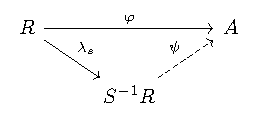
\includegraphics[scale = 1]{cd.pdf}
                  \end{center}

        \end{enumerate}
    \end{definition}

    Как и всегда, определение объекта через универсальное свойство ничего не говорит о существовании объекта, поэтому
    сейчас мы будем больно и мучительно строить локализацию.\\

    \textbf{Построение локализации:}\\

    Определим отношение $\sim$ на множестве $R \times S$ по правилу
    \[ (r_1, s_1) \sim (r_2, s_2) \Longleftrightarrow s s_2 r_1 = s s_1 r_2 \]
    \begin{remark}
        Здесь мы домножаем на $s$ как раз за тем, чтоб делители нуля ушли в ноль.
    \end{remark}
    \begin{statement}
        $\sim$~--- отношение эквивалентности.
    \end{statement}
    \begin{proof}
        Рефлексивность и симметричность очевидны. \\
        Самое неприятное~--- транзитивность.\\
        Пусть $(r_1, s_1) \sim (r_2, s_2)$ и $(r_2, s_2) \sim (r_3, s_3)$, то есть
        \[ s r_1 s_2 = s r_2 s_1, \quad s' r_2 s_3 = s' r_3 s_2, \ s, s' \in S \]
        Домножим первое равенство $s' s_3$, а второе $s s_1$, получим
        \[ s r_1 s_2 = s r_2 s_1 \to s' s_3 s r_1 s_2 = \textcolor{blue}{s' s_3 s r_2 s_1}, \qquad s' r_2 s_3 = s' r_3 s_2 \to \textcolor{blue}{s s_1 s' r_2 s_3}  = s s_1 s' r_3 s_2 \]
        Остается заметить, что
        \[ s s' s_2 \in S \Rightarrow (r_1, s_1) \sim (r_3, s_3) \]
        то есть, транзитивность доказана.
    \end{proof}

    Теперь, положим $S^{-1}R = R \times S / \sim$. Класс эквивалентности, содержащий представитель $(r, s)$ будем обозначать
    $\frac{r}{s}$.\\
    Определим локализационный гомоморфизм $\lambda_s\colon R \to S^{-1}R$ формулой $\lambda_{S}(r) = \frac{r}{1}$.\\

    \textcolor{blue}{Теперь, научимся складывать дроби.}

    \begin{theorem}
        Пусть $S$~--- мультипликативное подмножество кольца $R$. Определим на $S^{-1}R$ операции следующим образом
        \[ \frac{r_1}{s_1} \cdot \frac{r_2}{s_2} = \frac{r_1 r_2}{s_2 s_2}, \quad \frac{r_1}{s_1} + \frac{r_2}{s_2} = \frac{s_1 r_2 + s_2 r_1}{s_1 s_2} \]
        Тогда $S^{-1}R$~--- локализация $R$ в мультипликативном подмножестве $S$ с локализицонном гомоморфизмом $\lambda_s$ (как написано выше).
    \end{theorem}
    \begin{proof}
        Докажем сначала, что наше определение сложения и умножения не зависит от выбора представителя. \\
        Пусть выплняются равенства
        \[ \frac{r_1'}{s_1'} = \frac{r_1}{s_1} \leftrightarrow s r_1 s_1' = s r_1' s_1, \quad \frac{r_2'}{s_2'} = \frac{r_2}{s_2} \leftrightarrow s' r_2 s_2' = s' r_2' s_2 \]
        Перемножим последние равенства
        \[ s s' r_1 s_1' r_2 s_2' = s s' r_1' s_1 r_2' s_2 \]
        Отсюда имеем
        \[ \frac{r_1 r_2}{s_1 s_2} = \frac{r_1' r_2'}{s_1' s_2'} \]
        Далее, будет некоторая \textcolor{red}{боль}, а именно, надо доказать
        \[ \frac{r_1 s_2 + r_2 s_1}{s_1 s_2} = \frac{r_1' s_2' + r_2' s_1' }{s_1' s_2'} \]
        Если Вы немного помедитируете на формулы ниже, станет понятно, почему это так:
        \[ ss' (r_1 s_2 + r_2 s_1) s_1' s_2' = s s' (e_1 s_2 s_1' s_2' + r_2 s_1 s_1' s_2') =
        s s' (r_1' s_2 s_1 s_2' + r_2' s_1 s_2' s_2) = s s' (r_1' s_2' + r_2' s_1') s_1 s_2 \]
        Вообще, честно говоря, также нужно доказывать ассоциативность сложения, коммутативность и дистрибутивность.
        Давайте непосредственно проврим ассоциативность сложения
        \[ \left( \frac{r_1}{s_1} + \frac{r_2}{s_2} \right) + \frac{r_3}{s_3} = \frac{r_1 s_2 + r_2 s_1}{s_1 s_2} + \frac{r_3}{s_3} = \frac{r_1 s_2 s_3 + r_2 s_1 s_3 + r_3 s_1 s_2}{s_1 s_2 s_3} \]
        \[ \frac{r_1}{s_1} + \left( \frac{r_2}{s_2} + \frac{r_3}{s_3} \right) = \frac{r_1}{s_1} + \frac{r_2 s_3 + r_3 s_2}{s_2 s_3} = \frac{r_1 s_2 s_3 + r_2 s_3 s_1 + r_3 s_2 s_1}{s_1 s_2 s_3}\]
        Нейтральным элементом по сложению будет $\frac{0}{1} = \frac{0}{s}$, обратным по сложению к $\frac{r}{s}$~--- $-\frac{r}{s}$.
        Нейтральным элементом по умножению~---$\frac{1}{1} = \frac{s}{s}$. Проверим свочтва локализации:
        \[ \lambda_s(s) \cdot \frac{1}{s} = \frac{s}{1} \cdot \frac{1}{s} = 1 \]
        то есть, первое свойство выполнено. \\

        Пусть $\varphi\colon R \to A$~--- такой гомоморфизм колец, что $\varphi(s) \in A^* \ \forall s \in S$.
        Определим отображение $\psi\colon S^{-1}R \to A$ равенством $\psi(\frac{r}{s}) = \varphi(r) \varphi(s)^{-1}$. \\

        Если $\frac{r'}{s'} = \frac{r}{s}$, то по определению
        \[ \frac{r'}{s'} = \frac{r}{s} \Leftrightarrow r' s = r s', \ s'' \in S \Rightarrow \varphi(s'')\varphi(r')\varphi(s) = \varphi(s'') \varphi(r) \varphi(s') \]
        Домножим на $\varphi(s'')^{-1} \varphi(s')^{-1} \varphi(s')^{-1}$, получим
        \[ \varphi(r') \varphi(s')^{-1} = \varphi(r) \varphi(s)^{-1} \]
        а значит, $\psi$ определён корректно. Так как $\varphi(1) = 1$, имеем $\varphi = \psi \circ \lambda_{S}$. Ясно, что $\psi$~--- гомоморфизм. \\

        Равенство $\varphi = \psi \circ \lambda_{S}$ однозначно задаёт $\psi(\frac{r}{1}) = \varphi(r)$. Так как $\psi$ должен
        быть гомоморфизмом,
        \[ \varphi(r) = \psi(\frac{r}{1}) = \psi(\frac{r}{s} \cdot \frac{s}{1}) = \psi(\frac{r}{s}) \cdot \varphi(s) \]
        Так как по условию $\varphi(s) \in A^*$, имеем $\psi(\frac{r}{s}) = \varphi(r)\varphi(s)^{-1}$, что завершает доказательство.


    \end{proof}

    \textsc{\textbf{Примеры локализации:}}
    \begin{enumerate}
        \item Для $s \in R$ положим $\langle s \rangle = \{ s^n \ | \ n \in \mathbb{N} \}$. Локализация $\langle s \rangle^{-1}R$
              обозначается через $R_s$ и называется главной локализацией в элементе $s$ (по аналогии с главным идеалом).
        \item Если $P$~--- простой идеал кольца $R$, то $R \setminus P$ является мультипликативным подмножеством.
              В этом случае локализация $R_{P} = (R \setminus P)^{-1} R$ называется локализацией $R$ в простом идеале $P$.
              $R_P$ является локальным кольцом (т.е. кольцом с единственным максимальным идеалом).
        \item $S$~--- множество всех элементов $R$, не являющийся делителями нуля. Тогда $S^{-1}R$ называется полным кольцом частных
              кольца $R$. Это максимальная локализация, для которой гомоморфизм локализации инъективен.
    \end{enumerate}

    Если $R$~--- область целостности, то $\{ 0 \}$~--- простой идеал. Локализация в этом идеале, очевидно,
    будет полем, которое называется полем частных кольца $R$.\\

    Иными словами, поле частных~--- это полное кольцо частных области целостности. Локализационный гомоморфизм~--- это
    универсальное вложение в следующем смысле:

    \begin{lemma}
        Пусть $R$~--- область целостности, а $S = R\seminus \{ 0 \}$. Тогда $F = S^{-1}R$ является полем, а гомоморфизм
        локализации $\lambda_{S}\colon R \to F$ инъективен, а $\lambda_{S}$ удовлетворяет следующему универсальному свойству:
        для любого поля $K$ и мономорфизма $R \to K$ существует единственный мономорфизм $\psi\colon F \to K$, что $\varphi = \psi \circ \lambda_s$.
    \end{lemma}

    \subsection{Поле $p$-адических чисел, как поле частных кольца $\mathbb{Z}_p$.}

    Как мы уже выяснили, кольцо $\mathbb{Z}_p$~--- область целостности, его можно вложить в поле частных, используя
    конструкцию локализации.\\
    В нашем случае это сводится к рассмотрению дробей $\alpha / p^k$, где $\alpha \in \mathbb{Z}_p, \ k \ge 0$.
    \begin{definition}
        Дробь вида $\alpha / p^k$, где $\alpha \in \mathbb{Z}_p$, а $k \ge 0$ называется дробным $p$-адмическим числом
        или просто $p$-адическим числом.
    \end{definition}
    \begin{remark}
         Две дроби $\alpha / p^k$ и $\beta / p^m$ определяют одно и то же $p$-адическое число, если $\alpha p^m = \beta p^k$.
    \end{remark}

    \begin{definition}
        Полем  $p$-адических чисел $\mathbb{Q}_p$ называется поле частных кольца целых $p$-адических чисел $\mathbb{Z}_p$.
    \end{definition}

    \begin{theorem}
        Всякое $p$-адическое число $\xi \neq 0$ единственным образом представляется в виде
        \[ \xi = p^m \cdot \varepsilon, \quad m \in \mathbb{Z}, \ \varepsilon \in \mathbb{Z}_p^{*} \]
    \end{theorem}
    \begin{proof}
        Пусть $\xi = \alpha / p^k, \ \alpha \in \mathbb{Z}_p$. По теореме \ref{predstp-adic}  $\alpha$ можно представить в виде
        $p^{\ell} \varepsilon, \ \ell \ge 0, \varepsilon \in \mathbb{Z}_p^{*}$. Тогда $\xi = p^m \varepsilon, m = \ell - k$.\\
        Единственность вытекает из единственности представления для \ref{predstp-adic}.
    \end{proof}

    \subsection{Сходимость в поле $p$-адических чисел}
    Мы уже много раз говорили об аналогии между $p$-адическими числами и вещественными. В случае вещественных, они определяются последовательностями
    рациональных и являются пределами этих последоватлеьностей. \\

    Неформально мы уже обсуждали, почему это так в случае $p$-адических чисел, давайте теперь поймем, почему это так формально. \\

    Теперь, после того как мы доопределили $p$-адический показатель на $\mathbb{Q}_p$, мы можем вводить на $\mathbb{Q}_p$ (заметьте, уже не на $\mathbb{Q}$) знакомое
    нам  $p$-адическое нормирование (и, соответственно, $p$-адическую метрику).

    \begin{definition}
        Последовательность $p$-адических чисел $\{ \xi_n \}$ называется сходящейся к $p$-адическому числу  $\xi$ если
        \[ \lim\limits_{n \to \infty} \upsilon_p(\xi_n - \xi) = \infty \]
    \end{definition}
    \begin{remark}
        Ясно, что эквивалентно сходимость можно определять, как
        \[ \lim\limits_{n \to \infty} \{ \xi_n \} = \xi \Leftrightarrow \lim\limits_{n \to \infty}\| \xi_n - \xi \| = 0\]
        то есть, как и обычно, начиная с некоторого довольно большого номера, $p$-адические числа становятся сколь угодно близки к пределу.
    \end{remark}
    Рассмотрим сначала для удобства некоторые свойства $p$-адического показателя:
    \begin{enumerate}
        \item $\upsilon_{p}(\alpha \beta) = \upsilon_p(\alpha) + \upsilon_p{(\beta)} $.

        \item $ \upsilon_p{(\alpha + \beta)} \ge \min(\upsilon_p{(\alpha)}, \upsilon_p{(\beta)})$.

        \item $ \upsilon_p{(\alpha + \beta)} = \min{( \upsilon_p{(\alpha)}, \upsilon_p{(\beta)})}, \ \alpha \neq \beta$.
    \end{enumerate}
    Для поля $\mathbb{Q}_p$ справедливы все стандартные свойства пределов. Докажем, например, что при $\{ \xi_n \} \to \xi, \ \xi \in \mathbb{Z}_p^{*}$ выполняется $\{ 1 / \xi_n \} \to 1 / \xi_n$. \\

    Сначала отметим, что, начиная с некоторого места $ \upsilon_p{(\xi_n - \xi)} > \upsilon_p{(\xi)}$, откуда $ \upsilon_p{(\xi_n)} = \min( \upsilon_p{(\xi_n - \xi)}, \upsilon_p{(\xi)}) = \upsilon_p{(\xi)} \ \Rightarrow \upsilon_p{(\xi_n)} \neq \infty \Rightarrow \xi_n \neq 0$,
    то есть, на него в самом деле можно делить. \\

    Далее мы имеем
    \[ \upsilon_p{\left(\frac{1}{\xi_n} - \frac{1}{\xi} \right)} = \upsilon_p{(\xi - \xi_n)} - \upsilon_p{(\xi_n)} - \upsilon_p{(\xi)} = \upsilon_p{(\xi_n - \xi)} - 2v_p(\xi) \xrightarrow[n \to \infty]{} \infty \]
    Теперь, для доказательства факта, который мы хотели формализовать, нам нужно понять, как вводятся сравнения на кольце целых $p$-адических чисел.
    Сравнения в кольце целых $p$-адических чисел определяются также, как и в кольце целых чисел, то есть $\alpha \equiv \beta \pmod{\gamma} \Leftrightarrow (\alpha - \beta) \divisible \gamma$.\\

    Если $\gamma = p^n \varepsilon, \ \varepsilon \in \mathbb{Z}_p^{*}$, то всякое сравнение по модулю $\gamma$ равносильно сравнению по модулю $p_n$, а значит,
    достаточно рассматривать только такие (в этом случае).

    \begin{theorem}
        Всякое целое $p$-адическое число сравнимо с целым рациональным числом по модулю $p^n$. Два целых рациональных числа тогда и только тогда сравнимы по модулю
        $p^n$ в кольце $\mathbb{Z}_p^{*}$, когда они сравнимы по этому модулю в кольце $\mathbb{Z}$.
    \end{theorem}
    \begin{proof}
        Докажем сначала, что если $\alpha$~--- целое $p$-адическое число, определяемое последовательностью $\{ x_n \}$, то
        \[ \alpha \equiv x_{n - 1} \pmod{p^n} \]
        Как целое $p$-адическое число, $x_n$  определяется последовательностью $\{ x_n, x_n, \ldots, x_n, \ldots \}$. Тогда последовательность, определяющая целое $p$-адическое число
        $\alpha - x_n$ выглядит следующим образом
        \[ \{ x_0 - x_{n - 1}, \ x_1 - x_{n - 1}, \ldots, 0, x_n - x_{n - 1}, \ldots \}\]
        Из того, что всякое целое $p$-адическое число $\alpha$ представимо в виде
        \[ \alpha = p^k \cdot \varepsilon, \quad \varepsilon \in \mathbb{Z}_p^{*}\]
        следует, что целое $p$-адическое число $\alpha$, определяемое последовательностью $\{ y_n \}$ делится на $p^{\ell}$ тогда и только тогда, когда
        $x_n \equiv 0 \pmod{p^{n + 1}} \forall n = 0, 1, \ldots, k - 1$.
        Тогда, сравнение  $\alpha \equiv x_n \pmod{p^n}$ равносильно сравнениям
        \[ x_k - x_{n - 1} \equiv 0 \pmod{p^{k + 1}}, \ k = 0, 1, \ldots, n - 1\]
        а эти сравнения выполены по определению $p$-адических чисел.

        Докажем теперь, что для двух целых рациональных $p$-адических чисел $x$ и $y$ сравнимость по модулю $p^n$ в кольце $\mathbb{Z}_p$ равносильна
        сравнимости по модулю $p^n$ в кольце $\mathbb{Z}$.\\
        Положим $x - y = p^m a, \ a \not\equiv 0 \pmod{p} $. Тогда, в кольце $\mathbb{Z}$ сравнение $x \equiv y \pmod{p^n}$ равносильно условию $n \le m$.
        С другой стороны, так как $a \not\equiv - \pmod{p}$, соответсвующее ему целое $p$-адическое число обратимо в $\mathbb{Z}_p^{*}$, а значит, для числа
        $x - y$ есть представление в виде $p^m \alpha, \ \alpha \in \mathbb{Z}_p^{*}$, а значит, $ \upsilon_p{(x - y)} = m$, то есть, $n \le \upsilon_p{(x - y)}$,
        а в $\mathbb{Z}_p$ это равносильно сравнению $x \equiv y \pmod{p^n}$, так как $ \upsilon_p{(p^n)} = n$.
    \end{proof}
    \begin{theorem}
        Если целое $p$-адическое число $\alpha$ определяется последовательностью $\{ x_n \}$, то эта последовательность сходится к $\alpha$. Произвольное $p$-адическое число
        $\xi$ является пределом последовательности рациональных чисел.
    \end{theorem}
    \begin{proof}
        Как мы понимаем из предыдущей теоремы, если $\alpha \in \mathbb{Z}_p$ определяется последовательностью $\{ x_n \}$, то
        $\alpha \equiv x_{n - 1} \pmod{p^n}$, а это по определению влечёт $ \upsilon_p{(x_n - \alpha)}  \ge n + 1$. Значит, $ \upsilon_p{(x_n - \alpha)}  \xrightarrow[n \to \infty]{} \infty$,
        а это по определению означает, что $\{ x_n \}$ стремится к $\alpha$. \\

        Теперь рассмотрим дробное $p$-адическое число $\xi = \alpha / p^k$.
        \[ \upsilon_p{ \left( \frac{x_n}{p^k} - \xi)} \right) = \upsilon_p{\left( \frac{x_n - \alpha}{p^k}\right)} = \upsilon_p{(x_n - \alpha)} - k \xrightarrow[n \to \iinfty]{} \infty \]
        а значит, $\xi = \lim\limits_{n \to \infty} \{ y_n \}$, где $\{ y_n \} = \{ x_n / p^k \}$.\\

    \end{proof}

    \begin{definition}
        Последовательность $p$-адических чисел $\{ \xi_n \}$ называется ограниченной, если все значения $\| \xi \|_n$ ограничены сверху.
    \end{definition}

    \begin{theorem} \textbf{(Лемма Больцано-Вейерштрасса для поля $p$-адических чисел)}\\
        Из всякой ограниченной последовательности $p$-адических чисел можно извлечь сходящуюся подпоследовательность.
    \end{theorem}
    \begin{proof}
        Несложное, но не успеваю рассказать в курсе. Его можно найти в \textcolor{magenta}{\texttt{вставить ссылку на книжку Шафаревича в списке литературы.}}
    \end{proof}

    Оказывается (хоть это и не особенно неожиданно), для $p$-адических чисел справедлив критерий Коши, то есть

    \begin{theorem} \textbf{(Критерий Коши)}
        Пусть нам дана последовательность $\{ \xi_n \}, \ \xi_n \in \mathbb{Q}_p$. Тогда она сходится тогда и только тогда, когда
        \[ \lim\limits_{n, m \to \infty} \upsilon_p{(\xi_m - \xi_n)} = \infty \]
    \end{theorem}
    \begin{proof}
        Заметим, что из условия
        \[ \lim\limits_{n, m \to \infty} \upsilon_p{(\xi_m - \xi_n)} = \infty \]
        следует, что $\exists n_0 \colon \upsilon_p{(\xi_m - \xi_{n_0})} \ge 0 \ \forall m \ge n_0$.  Но тогда, по свойству $ \upsilon_p{(\alpha + \beta)} \ge \min(\upsilon_p{(\alpha)}, \upsilon_p{(\beta)})$.
        мы имеем
        \[ \upsilon_p{(\xi_m)} = \upsilon_p{((\xi_m - \xi_{m_0}) + \xi_{n_0})} \ge \min(0, \upsilon_p{(\xi_{n_0})}) \]
        а отсюда следует ограниченность. Значит, по предыдущей теореме, из неё можно извлечь сходящуюся попоследовательность $\{ \xi_{n_i} \}$ с пределом $\xi$.
        Значит, по определению сходимости $\exists N \in \mathbb{N}\colon \forall n, m \ge N \ \upsilon_p{(\xi_m - \xi_n)} \ge M $  и $ \upsilon_p{(\xi_{n_i} - \xi)} \ge M$
        Тогда
        \[ \upsilon_p{(\xi_m - \xi)} \ge \min( \upsilon_p{(\xi_m - \xi_{n_i}), \upsilon_p{(\xi_{n_i} - \xi)}}) \ge M \ forall m \ge N \]
        а значит $\lim\limits_{m \to \infty} \upsilon_p{(\xi_m - \xi)} = \infty$, то есть, последователньость $\{ \xi_m \}$ сходящаяся.
    \end{proof}

    В поле $p$-адических чисел этому признаку можно придать и более сильную форму. А именно, если для последоватльности $\{ \xi_n \}$
    выполенено
    \[ \lim\limits_{m, n \to \infty} \upsilon_p{(\xi_m - \xi_n)} = \infty\]
    то мы имеем и
    \[ \lim\limits_{n \to \infty} \upsilon_p{(\xi_{n + 1} - \xi_n)} = \infty\]
    Оказывается, что верно и обратное следствие. Действительно, если $\forall n \ge N \ \upsilon_p{(\xi_{n + 1} - \xi_n)} \ge M$, то в силу
    того, что $ \upsilon_p{(\alpha + \beta)} \ge \min(\upsilon_p{(\alpha)}, \upsilon_p{(\beta)})$  из равенства
    \[ \xi_m - \xi_n = \sum_{i - n}^{m - 1} (\xi_{i + 1} - \xi_i), \quad m > n \ge N  \]
    вытекает и оценка
    \[ \upsilon_p{(\xi_m - \xi_n)} \ge \min\limits_{i \in \{ n, \ldots, m - 1 \}} \upsilon_p{(\xi_{i + 1} - \xi_{i})} \ge M \Rightarrow \upsilon_p{(\xi_m - \xi_n)} \to \infty \]
    \begin{theorem}\label{p-adic_convergence}
        Для сходимости последовательности $p$-адических чисел $\{ \xi_n \}$ необходимо и достаточно, чтоб $\lim\limits_{n \to \infty} \upsilon_p{(\xi_{n + 1} - \xi_n)} = \infty$.
    \end{theorem}

    Ясно, что благодаря теории пределов мы можем определить секвенциальную непрерывность (непрерывность по Гейне) для функций $p$-адического аргумента. \\
    К тому же, ясны стандартные арифметические свойства непрерывных функций, из которых следует, например, что многочлен непрерывен.

    \begin{definition}
        Если последовательность частичных сумм $s_n = \sum\limits_{i = 0}^{n} \alpha_i$ ряда
        \[ \sum\limits_{i = 0}^{\infty} \alpha_i = \alpha_0 + \alpha_1 + \ldots + \alpha_n + \ldots \]
        c $p$-адическими членами сходится к $p$-адическому числу $\alpha$, то будем говорить, что ряд сходится и его сумма равна $\alpha$.
    \end{definition}

    Из теоремы  \ref{p-adic_convergence} можно легко получить критерий сходимости рядов из $p$-адических чисел.

    \begin{theorem} \textbf{(Критерий сходимости рядов с $p$-адическими членами)}\\
        Для сходимости ряда $\sum \alpha_n$ с $p$-адическими членами необходимо и достаточно, чтоб $\| \alpha_n \|_p \xrightarrow[n \to \infty]{} 0$ (или, что равносильно,
        $ \upsilon_p{(\alpha_n)} \xrightarrow[n \to \infty]{} \infty$).
    \end{theorem}
    \begin{proof}
        Действительно, мы имеем цепочку
        \[ s_n = \sum\limits_{k = 1}^n \alpha_k \text{~--- сходится} \Leftrightarrow \lim\limits_{n \to \infty} \| s_{n + 1} - s_n \|_{p} = 0 \Leftrightarrow \lim\limits_{n \to \infty} \left\| \sum\limits_{k = 0}^{n + 1} \alpha_k - \sum\limits_{k = 0}^{n} \alpha_k \right\|_p = \lim\limits_{n \to \infty} \| \alpha_{n + 1} \|_{p} = 0 \]
    \end{proof}

    Ясно, что как и в случае вещественного анализа, сходящиеся $p$-адические ряды можно складывать, умножать на константу.
    Также справедлива следующая теорема:
    \begin{theorem}
        При любой перестановке членов сходящегося $p$-адического ряда его сходимость не нарушается и сумма не меняется.
    \end{theorem}
    \begin{proof}
        Упражнение в листочке.
    \end{proof}
    Как мы знаем, в курсе вещественного (и комплексного) анализа это свойство характеризует абсолютно сходящиеся ряды. То есть, все сходящиеся
    $p$-адические ряды являются и абсолютно сходящимися, а значит, их можно и перемножать:
    \[ \text{написать сюда произведение рядов} \]

    Теперь уже ясно, что если целое $p$-адическое число $\alpha$ определяется канонической последовательностью $\{ x_n \}$, где
    \[ x_0 = a_0, \ x_1 = a_0 + a_1 p, \ x_2 = a_0 + a_1 p + a_2 p^2, \ldots, \ x_n = \sum\limits_{k = 1}^{n} a_n p^n \]
    то, так как мы доказали, что эта последовательность сходится к $\alpha$, а значит
    \[ \alpha = \lim\limits_{n \to \infty} \{ x_n \} = \lim\limits_{n \to \infty} \sum\limits_{k = 0}^{n} a_k p^k = \sum\limits_{k = 0}^{\infty} a_k p^k, \ 0 \le a_i < p \]
    Так как различные канонические последоватлеьности определяют различные $p$-адические числа, такое представление единственно для каждого числа.
    Представление целых $p$-адических чисел рядами напоминает запись вещественных чисел в виде бесконечных десятичных дробей, то есть
    \[ \overline{0, a_1 \ldots a_n \ldots } = \sum\limits_{k = 1}^{\infty} a_k \bigg(\frac{1}{10}\bigg)^k, \ 0 \le a_i < 10 \]
    Рассмотрим теперь ряд
    \[  b_0 + b_1 p + b_2 p^2 + \ldots + b_n p^n + \ldots, \ b_0 \in \mathbb{Z} \]
    то он будет сходящимся, так как $ \upsilon_p{(b_n p^n)} \ge n$, и его сумма будет равна некоторому $\alpha$.\\

    Для того, что бы для этого $\alpha$ получить каноническое представление, достаточно заменить все $b_i$ на $b_i \mod p$, относя неполное частное на каждом шаге к следующему
    члену. \\

    Это замечание актуально для действий в $\mathbb{Z}_p$, так как при сложении, вычитании и перемножении рядов вида $\sum a_k p^k, \ 0 \le a_i < p$, мы получаем ряды
    вида $\sum b_k p^k, \ b_k \in \mathbb{Z}$.
    Отметим, что в этом представлении, действия с $p$-адическими числами полностью аналогичны действиям с вещественными числами в десятичной записи.\\

    Из теоремы \ref{UnitP-adic} следует, что целое  $p$-адическое число, представленное в виде ряда обратимо тогда и только тогда, когда $a_0$. Вместе с теоремой \ref{predstp-adic}
    это даёт следующую теорему:

    \begin{theorem}
        Каждое отличное от нуля целое $p$-адическое число $\xi$ однозначно записывается ввиде
        \[ \xi = p^m(a_0 + a_1 p + a_2 p^2 + \ldots + a_n p^n + \ldots) \]
        где $m = \upsilon_p{(\xi)}, \ 1 \le a_0 \le p - 1, \ 0 \le a_n \le p - 1 \ \forall n \ge 2$.
    \end{theorem}
    Заметим, что эта запись соответсвует записи последовательности цифр, бесконечной влево, а именно
    \[ \alpha = \begin{cases}  \ldots a_{m + 1} a_m \overbrace{00\ldots0_{(p)}}^{m - 1}, \ m \ge 0 \\
        \ldots a_1 a_0 a_{-1} \ldots a_{m(p)}, m < 0 \end{cases}\]

    \textbf{\textsc{$p$-адические числа, как проективный предел:}}\\
    Разобранное нами построение кольца целых $p$-адических чисел соотвествует более общей алгебраической конструкции. А именно, мы на пальцах разобрали конструкцию
    проективного предела обратного спектра топологических пространств, групп, колец (не важно чего, в общем).\\

    \textcolor{magenta}{\textsc{\texttt{Параграф на доработке :(}}}.

    Так вот, из нашего построения ясно, что кольцо $\mathbb{Z}_p$ является проективным пределом последовательности $\mathbb{Z}/p^n\mathbb{Z}$ с естественным отображением $\mathbb{Z}/p^n\mathbb{Z} \to \mathbb{Z}/p^m\mathbb{Z}$ <<взятие остатка>>.
    \[ \mathbb{Z}_p = \varprojlim \mathbb{Z}/p^n\mathbb{Z} \]
    
    \subsection{Лемма Гензеля:}

    \begin{definition}
        Числовым полем называют конечное расширение поля $\mathbb{Q}$.
    \end{definition}
    \begin{example}
        Например,  $\mathbb{Q}(\sqrt{2}), \ \mathbb{Q}(i)$~--- числовые поля. Поле $\mathbb{R}$ не является конечным расширением
        $\mathbb{Q}$, а значит, это не числовое поле.
    \end{example}
    \begin{definition}
        Элемент $\alpha$ расширения поля $\mathbb{Q}$ называется алгебраическим числом, если он является корнем ненулевого многочлена
        в $\mathbb{Q}[T]$.
    \end{definition}
    \begin{example}
        Например, $\frac{1}{2}, \sqrt{2}, i$~--- алгебраические числа. Числа $e, \pi$ не являются алгебраическими (доказателсьтва представили
        Эримт в 1873г. и Линдеманн в 1882г.).
    \end{example}
    \begin{definition}
        Элемент $\alpha$ поля, являющегося расширением $\mathbb{Q}$ называется алгебраическим целым, если он является корнем унитарного многочлена
        с целыми коэффицентами.
    \end{definition}
    \begin{definition}
        Все алгебраические целые элементы поля $K$ образуют кольцо, которое принято называть кольцом целых поля $K$ и обозначать $\mathcal{O}_{K}$.
    \end{definition}
    \begin{example}
        $\mathcal{O}_{\mathbb{Q}} = \mathbb{Z}, \ \mathcal{O}_{Q_{p}} = \mathbb{Z}_p$.
    \end{example}
    \begin{definition}
        Пусть $(F, \| \cdot \|)$~--- полное неархимедово нормированное поле. Обозначим за
        \[ \mathbb{Z}_{F} = B_1(0) = \{ x \in F \ | \ \| x \| \le 1 \} \]
        ~--- <<кольцо целых>> чисел поля $F$.
    \end{definition}

    \begin{theorem} \textbf{(Лемма Гензеля)}
        Пусть $f(x) \in \mathbb{Z}_{F}[x], \ \alpha_0 \in \mathbb{Z}_{F}$ и справедливо неравенство $\| f(\alpha_0) \| < \| f'(\alpha_0)\|^2$ (тут $f'$~--- формальная производная многочлена $f$).
        Тогда существует единственное $\alpha \in \mathbb{Z}_{F}$, такое, что $f(\alpha) = 0$ и $\| \alpha - \alpha_0\| < \| f'(\alpha_0) \|$.
    \end{theorem}
    \begin{proof}
        Положим $c = \| f(\alpha_0) \| / \| f'(\alpha_0)\|^2 < 1$. Рассмотрим рекуррентно заданную последовательность
        \[ \alpha_{n + 1} = \alpha_n - \frac{f(\alpha_n)}{f(\alpha_{n + 1})}, \ n \ge 0 \]
        (<<метод касательных Ньютона>>). \\
        Индукцией проверяется, что она обладает следующими свойствами:
        \begin{enumerate}
            \item $\| \alpha_n - \alpha_0 \| < c \| f'(0) \| < \| f'(\alpha_0) \|$.
            \item $\| f'(\alpha_n)\| = \| f'(\alpha_0)\|$.
            \item $\| f(\alpha_n) \| \le c^{2^n} \| f(\alpha_0) \|^2$.
            \item $\| \alpha_n - \alpha_0 \| \le c^{2^n} \| f(\alpha_0) \|$.
        \end{enumerate}

        А значит, можно взять $\alpha = \lim\limits_{n \to \infty} \alpha_n$.
        Единственность следует из разложения многочлена по тейлору в точке $\alpha$.
    \end{proof}
    \begin{corollary} \textbf{(Важное:)} \\
         Пусть $f \in \mathbb{Z}_p[x], \ \alpha_0 \in \mathbb{Z}_p,\ f(\alpha_0) \equiv 0 \pmod{p}, \ f'(\alpha_0) \not\equiv 0 \pmod{p}$.
        Тогда существует единственное $\alpha \in \alpha_0 + p\mathb{Z}_p$ такое, что $f(\alpha) = 0$.
     \end{corollary}

    Кроме того, есть еще \textsc{народная} формулировка леммы Гензеля:
    \begin{theorem}
        Пусть $f$~--- многочлен с целыми (или целыми $p$-адическими коэффицентами), а $m$ и  $k$~--- целые числа, причем
        $0 \le m \le k$. Тогда, если $r$~--- целое число, такое, что
        \[ f(r) \equiv 0 \pmod{p^k}, \ f'(r) \neq 0 \pmod{p} \]
        то существует такое целое $s$, что
        \[ f(s) \equiv 0 \pmod{p^{k + m}}, \  r \equiv s \pmod{p^k} \]
        и более того, $s$ может быть выражено в явном виде, а именно,
        \[ s = r - f(r) \cdot a, \ a = (f(r))^{-1} \pmod{p^m}\]

    \end{theorem}

    \subsection{Пополнение метрических пространств.}

    \begin{definition}
    Пусть $(X, d_X)$~--- метрическое пространство, $\mathcal{F}(X)$~--- множество всех ограниченных функций из $X$ в $\mathbb{R}$. Тогда введём расстояние $d_{\infty}$ между функциями $f, g \in \mathcal{F}(X)$:
    \begin{equation*}
        d_{\infty}(f, g) \eqdef \sup\{|f(x) - g(x)|, x \in X\}
    \end{equation*}
    Заметим, что определение корректно, так как функции ограничены.
    \end{definition}

    \begin{lemma}

    $(\mathcal{F}(X), d_{\infty})$~--- метрическое пространство.

    \end{lemma}

    \begin{proof}

     Проверим три аксиомы метрики:
    \begin{enumerate}
        \item Пусть $f = g$. Тогда $|f(x) - g(x)| = 0$ для всякого $x \in X$, так что $d_{\infty}(f, g) = 0$. Если же наоборот $d_{\infty}(f, g) = 0$, то $0 \leq |f(x) - g(x)| \leq \sup = 0$, а значит $f(x) = g(x)$ для всех $x \in X$, что и означает $f \equiv g$.
        \item Так как $|f(x) - g(x)| = |g(x) - f(x)|$, то и $d_{\infty}(f, g) = d_{\infty}(g, f)$.
        \item Рассмотрим три ограниченные функции $f, g, h \in \mathcal{F}(X)$, и покажем, что
        \begin{equation*}
            d_{\infty}(f, g) + d_{\infty}(g, h) \geq d_{\infty}(f, h)
        \end{equation*}
        Мы знаем, что:
        \begin{equation*}
            \forall x \in X: |f(x) - g(x)| + |g(x) - h(x)| \geq |f(x) - h(x)|
        \end{equation*}
        в силу неравенства треугольника для стандартной метрики на $\mathbb{R}$. Для всякого $\varepsilon > 0$ мы можем взять $x_0$ такой, что $|f(x_0) - h(x_0)| \geq \sup\{|f(x) - h(x)|, x \in X\} - \varepsilon$. Получаем, что
        \begin{equation*}
            d_{\infty}(f, h) - \varepsilon = \sup\{|f(x) - h(x)|, x \in X\} - \varepsilon \leq |f(x_0) - h(x_0)| \leq
        \end{equation*}
        \begin{equation*}
            \leq |f(x_0) - g(x_0)| + |g(x_0) - h(x_0)| \leq d_{\infty}(f, g) + d_{\infty}(g, h)
        \end{equation*}
        а раз это верно для любого $\varepsilon > 0$, то искомое неравенство доказано.
    \end{enumerate}
    \end{proof}

    \begin{lemma}
    $\mathcal{F}(X)$~--- полно.
    \begin{proof}
    Пусть $f_{n}$~--- фундаментальная последовательность функций. Тогда $\forall x_0 \in X: \{f_{n}(x_0)\}$~--- также фундаментальная последовательность, так как $|f_{n}(x_0) - f_{m}(x_0)| \leq \sup\{|f_{n}(x) - f_{m}(x)|, x \in X\}$. Следовательно,
    \begin{equation*}
        \forall x_0 \in X: \exists \lim_{n \to \infty} f_{n}(x_0)
    \end{equation*}
    и сходимость по всем точкам равномерна, так как не зависит от выбора точки $x_0$. Иными словами,
    \begin{equation*}
        \exists f(x): \forall \varepsilon > 0: \exists N: \forall n > N: d_{\infty}(f_n, f) < \varepsilon
    \end{equation*}
    где $f(x_0)$ определяется как предел $ \lim_{n \to \infty} f_{n}(x_0)$. Так что $f(x)$~--- функция, являющаяся пределом искомой последовательности функций.
    \end{proof}
    \end{lemma}

    \begin{definition}
    Пусть $(X, d_X)$~--- метрическое пространство, $\mathcal{F}(X)$~--- множество ограниченных функций из $X$ в $\mathbb{R}$. Построим изометрическое вложение $k: X \to \mathcal{F}(X)$ следующим образом:
    \begin{enumerate}
        \item Если $X$~--- ограничено, то определим $k(x) = d_x$, где
        \begin{equation*}
            \forall y \in X: d_x(y) \eqdef d_X(x, y)
        \end{equation*}
        Функция $d_x$ ограничена, так как $X$ ограничено. Заметим также, что
        \begin{equation*}
            d_{\infty}(d_x, d_y) = \sup_{z} |d_x(z) - d_y(z)| = \sup_z \big( d_X(x, z) - d_X(z, y) \big) \leq d_X(x, y)
        \end{equation*}
        однако равенство достигается при $z = y$, так что $d_{\infty}(d_x, d_y) = d_X(x, y)$, а значит вложение изометрическое.
        \item Пусть $X$, возможно, не ограничено. Тогда определим $k(x) = d_x - d_{x_0}$ для некоторой фиксированной точки $x_0 \in X$, где
        \begin{equation*}
            \forall y \in X: \big(k(x)\big)(y) \eqdef d_x(y) - d_{x_0}(y) = d_X(x, y) - d_X(y, x_0)
        \end{equation*}
        что есть ограниченная функция, так как $\forall y \in X: d_X(x, y) - d_X(y, x_0) \leq d_X(x, x_0)$. \\
        Заметим, что это аналогичным образом будет изометрическим вложением:
        \begin{equation*}
            d_{\infty}(d_x - d_{x_0}, d_y - d_{x_0}) = \sup_{z} |d_x(z) - d_{x_0}(z) - d_y(z) + d_{x_0}(z)| =
        \end{equation*}
        \begin{equation*}
            = \sup_z \big( d_X(x, z) - d_X(z, y) \big) \leq d_X(x, y)
        \end{equation*}
        где равенство достигается при $z = y$.
    \end{enumerate}
    \end{definition}

    \begin{Theorem}
    Любое метрическое пространство $(X, d_X)$ имеет пополнение $(\overline{X}, d_{\overline{X}})$, то есть такое метрическое пространство $\overline{X}$, что выполнено:
    \begin{enumerate}
        \item $X \subseteq \overline{X}$
        \item $X$~--- всюдю плотно в $\overline{X}$
        \item $d_{\overline{X}}|_X = d_X$, то есть вложение из $X$ в $\overline{X}$ является изометрическим
        \vspace{3pt}
        \item $(\overline{X}, d_{\overline{X}})$~--- полно.
    \end{enumerate}
    \end{Theorem}
    \begin{proof}
    Возьмём изометрическое вложение Куратовского $k: X \to \mathcal{F}(X)$, и возьмём его замыкание в топологическом пространстве $\mathcal{F}(X)$ с топологией, индуцированной метрикой $d_{\infty}$~--- назовём это замыкание $\overline{X}$. Заметим, что
    \begin{enumerate}
        \item $X \subseteq \overline{X}$ естественным образом
        \item $X$ всюду плотно в $\overline{X}$, так как любое множество всюду плотно в своём замыкании
        \item Вложение $X$ в $\overline{X}$ изометрическое, так как оно изометрическое и во всё пространство $\mathcal{F}(x)$
        \item $\overline{X}$ полно как замкнутое подмножество полного пространства.
    \end{enumerate}
    \end{proof}


    \begin{remark}
    Пополнение метрического пространства \textbf{единственно} с точностью до изометрии.
    \end{remark}

    \begin{remark}
    Выражение $X \subseteq \overline{X}$ тоже подразумевается с точностью до изометрии.
    \end{remark}
    \subsection{Пополнение нормированного поля.}
    Теперь мы умеем пополнять метрические пространства, но нам никто не гарантирует, что при пополнении поля по норме получится поле.
    \begin{definition}
        Пополнением нормированного поля $(F_0, \| \cdot \|_0 )$ называется нормированное поле $(F, \| \cdot \|)$,
        уловлетворяющее следующим свойствам
        \begin{enumerate}
            \item Существует вложение $i\colon F_0 \hookrightarrow F$, сохраняющее норму (изометрическое), то есть $\| i(x) \| = \| x \|_0$.

            \item $(F, \| \cdot \|)$ полно, как метрическое пространство.

            \item $i(F_0)$ всюду плотно в $F$, то есть, $\forall x,  \varepsilon > 0 \ \exists x_0 \in F_0\colon \| x - i(x_0)\| < \varepsilon$.
        \end{enumerate}
    \end{definition}

    \begin{example}
        Из курса анализа ясно, что $(\mathbb{R}, |\cdot|)$~--- пополнение $(\mathbb{Q}, |\cdot|)$.
    \end{example}

    \begin{theorem}
        Для любого нормированного поля существует пополнение.
    \end{theorem}
    \begin{proof}
        Будем рассматривать случай нормы с неравенством треугольника. \\
        Пусть $\mathfrak{A}$~--- множество всех последовательностей Коши $\{ x_n \}_{n = 1}^{\infty}$ в пространстве
        $(F_0, \| \cdot \|_0)$.\\
        На $\mathfrak{A}$ можно естествнным образом определить операции сложения и умножения (поточечно), а также ввести норму $\| \cdot \|$, как
        $\| \{ x_n \} \| = \lim\limits_{n \to \infty} \| x_n \|_{0}$.\\
        Это определение корректно, так как предел всегда существует в силу неравенства треугольника и того, что $\{ x_n \}$~---
        последовательность Коши
        \[ |\| x_n \|_0 - \| x_m \|_0 | \le \| x_n - x_m \|_0 \]
        Ясно, что остальные свойства нормы также выполняются. \\

        Введём на $\mathfrak{A}$  отношение эквивалентности $\sim$:
        \[ \{ x_n \} \sim \{ y_n \} \Leftrightarrow \lim\limits_{n \to \infty} \| x_n - y_n \|_0  = 0 \]
        Нетрудно заметить, что это отношение эквивалентности <<уважает>> арифметические действия и норму, то есть
        \begin{enumerate}
            \item $\{ x_n \} \sim \{ u_n \}, \ \{ y_n \} \sim \{ v_n \} \Rightarrow \{ x_n + y_n \} \sim \{ u_n + v_n \}$, $\{ x_n y_n \} \sim \{ u_n v_n \}$.
            \item $\{ x_n \} \sim \{ y_n \} \Rightarrow \| \{ x_n \} \| = \| \{ y_n \} \|$.
        \end{enumerate}

        В качестве поля $F$ возьмем фактормножество $\mathfrak{A}/\sim$. Приведенные выше свойства естественно индуцируют арифметические операции и норму
        с $\mathfral{A}$ на $F$:
        \begin{itemize}
            \item $[\{ x_n \}] + [\{ y_n \}] = [\{ x_n + y_n \}]$.
            \item $[\{ x_n \}] \cdot [\{ y_n \}] = [\{ x_n \cdot y_n \}]$.
            \item $\| [\{ x_n \}] \| = \| \{ x_n \}\|$.
        \end{itemize}
        Аксиомы кольца вполне очевидны, проверим существование обратного по умножению элемента.
        Если $[\{ x_n \}] \neq 0$, то $\lim \| x_n \|_0 > 0 \Rightarrow \forall n \ge n_0 \ \| x_n \|_0 > \delta > 0$ для
        некоторого $\delta$.

        Тогда в качестве $[\{ x_n \}]^{-1}$ возьмем класс $[\{ y_n \}]$, где
        \[ y_n = \begin{cases} 0,\quad n < n_0 \\ \frac{1}{x_n}, \quad n \ge n_0 \end{cases}\]

        Осталось проверить, что мы получили пополнение. \\
        В качестве вложения возьмем $i(x) = [(x, x, \ldots)]$. Ясно, что $i(F_0)$ плотно в $F$, так как, если
        $X = [\{ x_n \}] \in F$, то $i(x_n) \to X$ в пространстве $(F, \| \cdot \| )$.

        Теперь проверим полноту. Пусть $X^{(n)} = [( x_1^{(n)}, x_2^{(n)}, \ldots ) ] \in F$~--- последовательность Коши.
        Возьмем такую последовательность $k_n \in \mathbb{N}$, что
        \[ \sup\limits_{k, \ell \ge k_n} \| x_k^{(n)} = x_{\ell}^{(n)}\|_0 < \frac{1}{n} \]

        Покажем, что в качестве предела можно взять $X = [ \{ x_{k_n}^{(n)} \}]$. Пусть $N \ge k_n, \ M \ge k_m, \ K \ge \max\{ k_n, k_m \}$.
        \[ \| x_N^{(n)} - x_M^{(m)}\|_0 \le \| x_N^{(n)} - x_K^{(n)}\|_0 + \| x_K^{(n)} - x_K^{(m)}\|_0 \le \frac{1}{n} + \| x_K^{(n)} - x_K^{(m)}\|_0 + \frac{1}{m} \]

        Устремим $K$ к бесконечности и получим
        \[ \| x_N^{(n)} - x_M^{(m)} \|_0 \le \| X^{(n)} - X^{(m)}\| + \frac{1}{n} + \frac{1}{m} \]
        Положим $N = k_{n}, \ M = k_m$ и получим, что $x_{k_n}^{(n)}$~--- последовательность Коши, а её класс эквивалентности~--- искомый предел.
    \end{proof}

    Далее отождествим $i(F_0)$ с $F_0$ и будем считать, что $F \subseteq F$.\\

    В неархимедовом случае можно сказать даже несколько больше.

   Пусть $(F, \| \cdot \|)$~--- неархимедово нормированное поле. Если  $\{ x_n \} \to x, \ x \in F^{*}$, то для достаточно больших
    $n$ $\| x_n \| = \| x \|$.

   \begin{lemma}
       Пусть $(F, \| \cdot \|)$~--- пополнение неархимедова поля $(F_0, \| \cdot \|_0)$. Тогда
       \begin{enumerate}
           \item $(F, \| \cdot \|)$ неархимедово.

           \item $\Im(\| \cdot \|) = \Im(\| \cdot \|_0)$.
       \end{enumerate}
   \end{lemma}
    \section{Введение в алгебраическую геометрию}
    \subsection{Квадрики и рациональная параметризация квадрик.}
    \begin{definition}
        Пусть $X$~--- коммутативное кольцо и даны наборы коэффицентов $\{ a_i \} \in X$, $\{ b_i \} \in X, c \in X$.
        Если $\exists j\colon 1 \le j \le n, \ a_j \neq 0$.
        Квадратичной функцией (\textcolor{red}{не формой})  будем называть функцию вида
        \[ f(x_1, \ldots, x_n) = \sum\limits_{i, j = 1}^{n} a_{i} x_i x_j + \sum\limits_{i = 1}^{n} b_i x_i + c  \]
        Если $X$~--- аффинное пространство (мы будем считать, что векторное над полем $K$), то квадрикой мы будем называть множество нулей такой функции $X \to K$, то есть, множество вида
        \[ K = \{ x \in X \ | \ f(x) = f(x_1, \ldots, x_n) = 0 \]
    \end{definition}
    \begin{example}
        Эллипс, порабола и гипербола~--- известные вам квадрики на плоскости.
    \end{example}

    \begin{remark}
        Заметим, что если нам дана квадрика $M$, заданная, как множество нулей функции $f$ и мы сменили систему координат, то
        в новой системе координат $M$ также будет являться квадрикой, то есть, найдётся такая квадратичная функция $f'$, множеством нулей которой
        будет $M$.
    \end{remark}
    Часто нас будует интересовать,как выглядят квадрики над кольцом целых чисел, то есть, как решать диофантово уравнение
    $f(x_1, \ldots, x_m) = 0$. Эта задача весьма сложная, поэтому для начала попытаемся понять, как пытаться решать такие уравнения
    над полем $\mathbb{Q}$.

    \begin{example} Опишем все пифагоровы тройки, то есть, такие все тройки $(X, Y, Z) \in \mathbb{Z}^3$, что
        \[ X^2 + Y^2 = Z^2 \]
        Заметим, что достаточно описывать только тройки, где $\gcd(X, Y, Z) = 1$, так как, если мы умножим все три числа на какое-то
        целое число, то мы внось получим пифагорову тройку.

        Более того, достаточно рассматривать только тройки попарно взаимно простых чисел, так как
        \[ X \divisible p, \ Y \divisible p \Rightarrow X^2 + Y^2 = Z^2 \divisible p \]
        Заметим, что при $Z = 0$ мы имеем решение $(0, 0, 0)$, дальше будем рассматривать случаи $Z \neq 0$.
        Поделим на $z$ и получим уравнение
        \[ x^2 + y^2 = 1 \]
        То есть, мы свели задачу к перечислению всех рациональных точек на окружности.
        Некоторые рациональные точки $(0, \pm 1), \ (\pm 1, 0)$. Выберем из них, например, точку $A = (0, 1)$.
        Проведем всевозможные прямые через точку $A$ (кроме горизонтальных).
        Каждая такая прямая $\ell$ пересечет окружность еще в одной точке $B(x, y)$ и ось абсцисс в точке $C(c, 0)$.
        
        \begin{center}
            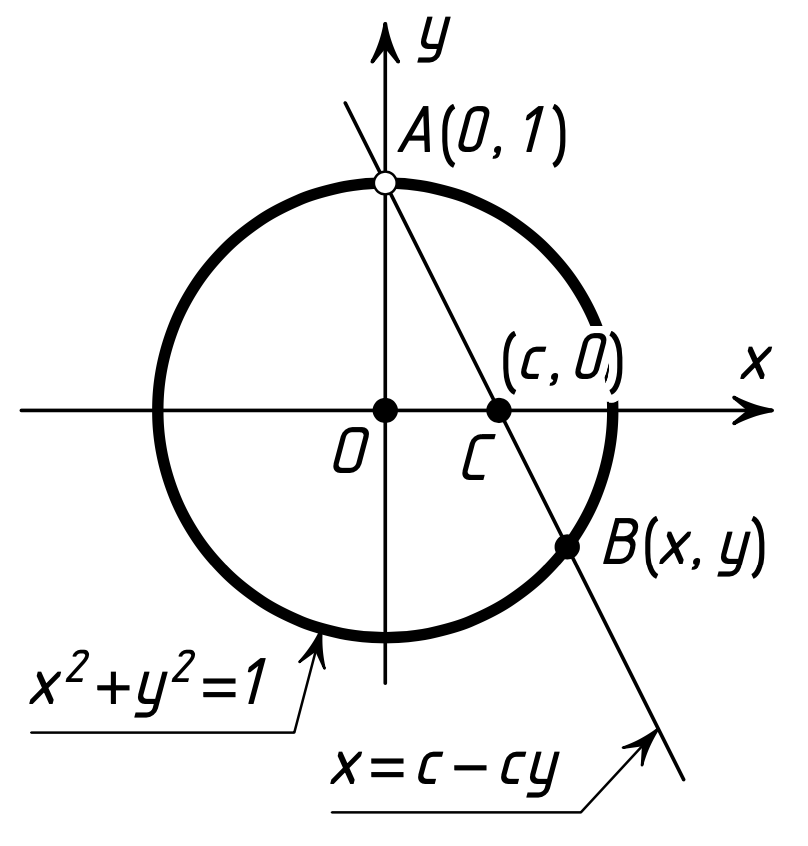
\includegraphics[scale = 0.2]{pic_1.png}
        \end{center}

        Таким обоазом, пересекая, мы получаем взаимнооднозначное соответствие между точками окружности и точками прямой.

        Причем, это соответствие сохраняет рациональность точек. Прямая, проходящая через точки $A$ и $C$ определяется
        уравнением $y = c - cy$. Подставим это в уравнение окружности
        \[ (c - cy)^2 + y^2 = 1 \Rightarrow  (c^2 + 1)y^2 - 2c^2 y + c^2 - 1 = 0 \]
        откуда мы имеем, что либо $y = 1$, либо $y = \frac{c^2 - 1}{c^2 + 1}$, при $x = c - cy = \frac{2c}{c^2 + 1}$.
        Остается заметить, что если $c \in \mathbb{Q}$, то $(x, y) \in \mathbb{Q}^2$. Обратное всегда вытекает Если координаты двух точек рациональны, то уравнение соединяющей их прямой можно записать так, чтобы оно имело рациональные коэффициенты.
        Если две прямые задаются уравнениями с рациональ- ными коэффициентами, то точка их пересечения (если она существует) имеет рациональные координаты.
        То есть, каждое рациональное решение, кроме $(0, 1)$ можно получить
        \[ x = \frac{2c}{c^2 + 1}, \quad y = \frac{c^2 - 1}{c^2 + 1} \]
        где $c \in \mathbb{Q}$. \\
        Подставим $c = m / n$, где $\gcd(m, n) = 1$, тогда
        \[ x = \frac{2c}{c^2 + 1} = \frac{2mn}{m^2 + n^2}, \quad y = \frac{c^2 - 1}{c^2 + 1} = \frac{m^2 - n^2}{m^2 + n^2}\]
        Теперь будем искать все целые решения, выполним обратную подстановку:
        \[ \frac{X}{Z} = \frac{2mn}{m^2 + n^2}, \quad \frac{Y}{Z} = \frac{m^2 - n^2}{m^2 + n^2}, \quad m^2 + n^2 \neq 0 \]
        Вспомним, что числа $(X, Y, Z)$ взаимно просты, а значит, дроби в левых частях несократимы. Если бы мы знали, что дроби, стоящие в правых частях тоже несократимы, то
        мы бы положили $X = 2mn$, $Y = m^2 - n^2, \ Z = m^2 + n^2$, но, к сожалению, они бывают сократимы.
        Но, они могут быть сократимы только на 2. Действительно, если $p$~--- простое число, не равное двум и $p \mid 2 mn$. Так как
        $\gcd(m, n) = 1$, если $p \mid m$, то $p \not\mid n \Rightarrow m^2 + n^2 \not\divisible p$, а значит, дробь $X / Z$ несократима.
        Рассмотрим теперь вторую дробь. Если $p$~--- простое число, не равное двум и $p \mid m^2 - n^2, \ p \mid m^2 + n^2$, то
        $p \mid 2m^2$ и $p \mid 2n^2$. Так как $\gcd(m, n) = 1$,  это влечёт $p = 2$. Итак, мы
        наконец нашли взаимнопростые натуральыне решения
        \[ X = mn, \ Y = \frac{m^2 - n^2}{2}, \ Z = \frac{m^2 + n^2}{2} \]
        при $\gcd(m, n) = 1$ и нечетных $m, n$, а также
        \[ X = 2mn, \ Y = m^2 - n^2, \ Z = m^2 + n^2 \]
        при взаимнопростых $m$ и $n$, одно из которых четно. Любые целые положительные решения мы получим умножением этих решений на натуральное число.
        Теперь заметим, что формулы для четного и нечетного случаев на самом деле совпадают.
        Если
        \[ X = pq,\  Y = \frac{p^2 - q^2}{2}, \ Z = \frac{p^2 + q^2}{2}\]
        ~--- решение, вычисленное по формулам для первого случая, где $\gcd(p, q) = 1$ и числа $p$ и $q$ оба нечетны, то те же решения
        мы получим и по вторым формулам, только подставляя
        \[ m = \frac{p + q}{2}, \quad n = \frac{p - q}{2} \]
        разве что с точностью до того, что $X$ и $Y$ поменяются местами.
    \end{example}

    \section{Проективная геометрия}
    \subsection{Модели построения проективной плоскости и связь между ними}
    \subsubsection*{Проективная плоскость, как факторпространство.}
    \begin{definition}
        Проективная плоскость $\mathbb{R}P^2$~--- факторпространство сферы по $x \sim -x$ (отождествление противоположных точек). \textbf{Прямая} в проективной плоскости~--- образ большой окружности сферы при проекции.
    \end{definition}

    \textbf{Свойство}: через любые две точки проходит ровно одна прямая. Любые две прямые пересекаются ровно по одной точке.

    \subsubsection*{Проективная плоскость и бесконечно удалённые точки.}

    Рассмотрим плоскость П (евклидову или аффинную, не важно). Определим
    \begin{definition}
        Назовём класс эквивалентности параллельных прямых бесконечно удалённой точкой.
    \end{definition}
    \begin{remark}
        Пополнение пространства $\Pi$ часто обозначают за $\widehat{\Pi}$.
    \end{remark}
    Тогда проективная плоскость $\widehat{\Pi}$~--- объединение П с множеством её бесконечно удалённых точек. Для каждой прямой $l \subseteq$ П определим проективную прямую $\hat{l}$~--- объединение $l$ и её бесконечно удалённой точки. Добавим в список прямых бесконечно удалённую прямую, состоящую из всех бесконечно удалённых точек.\\
    Верно, что через любые две точки проходит ровно одна прямая, и любые две прямых пересекаются в точности в одной точке.

    \subsubsection*{Соответствие между моделями}

    Возьмём П $\subseteq \mathbb{R}^3$, как плоскость не содержащую $0$. Будем проводить прямые через $0$ и пересекать их с плоскостью следующим образом:
    \begin{itemize}
        \item Если прямая пересекает нашу плоскость П, то ровно по одной точке. Её и сопоставим двум антиподальным точкам на сфере.
        \item Если она не пересекает плоскость П, то сопоставим данной паре точек бесконечно удалённую точку, соответствующую классу эквилинеарности прямых, параллельных данной.
    \end{itemize}

    \begin{remark}
        Таким образом, мы построили биекцию с сохранением свойств.
    \end{remark}
    \subsection{Проективные пространства и однородные координаты.}
    \begin{definition}
        $V$~--- векторное пространство. Проективное пространство, порождённое $V$~--- множество
        \begin{equation*}
            P(V) = (V \setminus \{0\}) \diagup_{\cong}
        \end{equation*}
        Где $\cong$~--- отношение пропорциональности: $x \cong y$, если найдётся такое $t \in \mathbb{R} \setminus \{0\}$, что $x = ty$.
    \end{definition}

    \begin{remark}
        Размерность $P(V)$ равна $\dim(V) - 1$ по определению.
    \end{remark}

    \begin{remark}
        \begin{enumerate}
            \item Можно считать, что $P(V)$~--- множество прямых в $V$ , проходящих через $O$.
            \item $P(\mathbb{R}^{n + 1}) \cong \mathbb{R}P^{n} = S^n \diagup_{x \cong -x}$
            \item Можно над любым полем, скажем, над $\mathbb{C}$ получим $\mathbb{C}P^m = P(\mathbb{C}^m)$
            \item Это проекция $p: V \setminus \{0\} \to P(V)$
        \end{enumerate}
    \end{remark}


    Пусть $(x_0, x_1, \hdots, x_n) \in \mathbb{R}^{n+1} \setminus \{0\}$, соответствующая ей точка в $P(x)$ обозначается как $[x_0 : x_1 : x_2 : \hdots : x_n]$. Они называются однородными координатами точки $P(x)$
. \\

    Два набора задают одну точку тогда и только тогда, когда они пропорциональны:
    \begin{equation*}
        [x_0 : \hdots : x_n] = [y_0 : \hdots : y_n] \Longleftrightarrow \exists c \in \mathbb{R} \setminus \{0\}: \ y_i = c \cdot x_i, \ \forall i
    \end{equation*}
    Например, $[1 : 2] = [3 : 6]$.

    \subsection{Проективное пополнение аффинного пространства}

    \begin{definition}
        Пусть $A$~--- аффинное пространство. Множество бесконечно удалённых точек $A_{\infty} = P(\overline{A})$. Тогда назовём проективным пополнением
        \begin{equation*}
            \hat{A} = A \sqcup A_{\infty}
        \end{equation*}
    \end{definition}

    На нём вводится структура проективного пространства: \\
    вкладываем $A$ в векторное пространство  $V$, $\dim(V) = \dim(A) + 1$ как гиперплоскость, не проходящую через $0$. Тогда $\overline{A}$ отождествляем с линейной гиперплоскостью в $V$ (которая, в свою очередь, проходит через $0$), строим биекцию $I: \hat{A} \to P(V)$ аналогично случаю сферы и проективной плоскости.

    \textbf{Свойства}:
    \begin{enumerate}
        \item $I$~--- биекция.
        \item $A_{\infty}$~--- гиперплоскость в $\hat{A}$, так называемая ``бесконечно удалённая гиперплоскость''
        \item Каждому аффинному подпространству $B \subseteq A$ соответствует проективное подпространство $\hat{B} \subseteq \hat{A}$.
        \item Существует контрпример к следующему утверждению: всякое проективное подпространство в $\hat{A}$ либо соответствует аффинному подпространству в $A$, либо содержится в бесконечно-удалённой гиперплоскости.
    \end{enumerate}
    \subsection{Проективное пополнение $\mathbb{R}^n$}

    Пусть у нас было $n$-мерное евклидово пространство $\mathbb{R}^n$, мы добавили к нему какие-то бесконечно удалённые точки
    и получили $\mathbb{R}P^n$. Топологически это просто компактификация, так как $\mathbb{R}^n$ не компактно, а $\mathbb{R}P^n$~--- сфера, у которой отождествили противоположные точки границы, то есть компакт.
    Выберем какую-то координатную систему в $ \mathbb{R}^n$ и выберем точку с координатами $(x_1, \ldots, x_n)$.
    Тогда, ей в $\mathbb{R}P^n$ будет соответствовать точка с вот такими координатами: $[x_1 : x_2 : \ldots : x_n : 1]$. Это так, потому что $\mathbb{R}P^n$~--- множество всех прямых, проходящих через 0 в $\mathbb{R}^{n + 1}$, то есть, мы можем взять $\mathbb{R}^n$ и вложить в $\mathbb{R}^{n + 1}$, как плоскость, задающуюся уравнением $x_{n + 1} = 1$. Тогда, каждой прямой, проходящей через 0 в $\mathbb{R}^{n + 1}$ будет соответствовать точка этой плоскости. \\
    \begin{center}
    \begin{figure}[h]
        \centering
        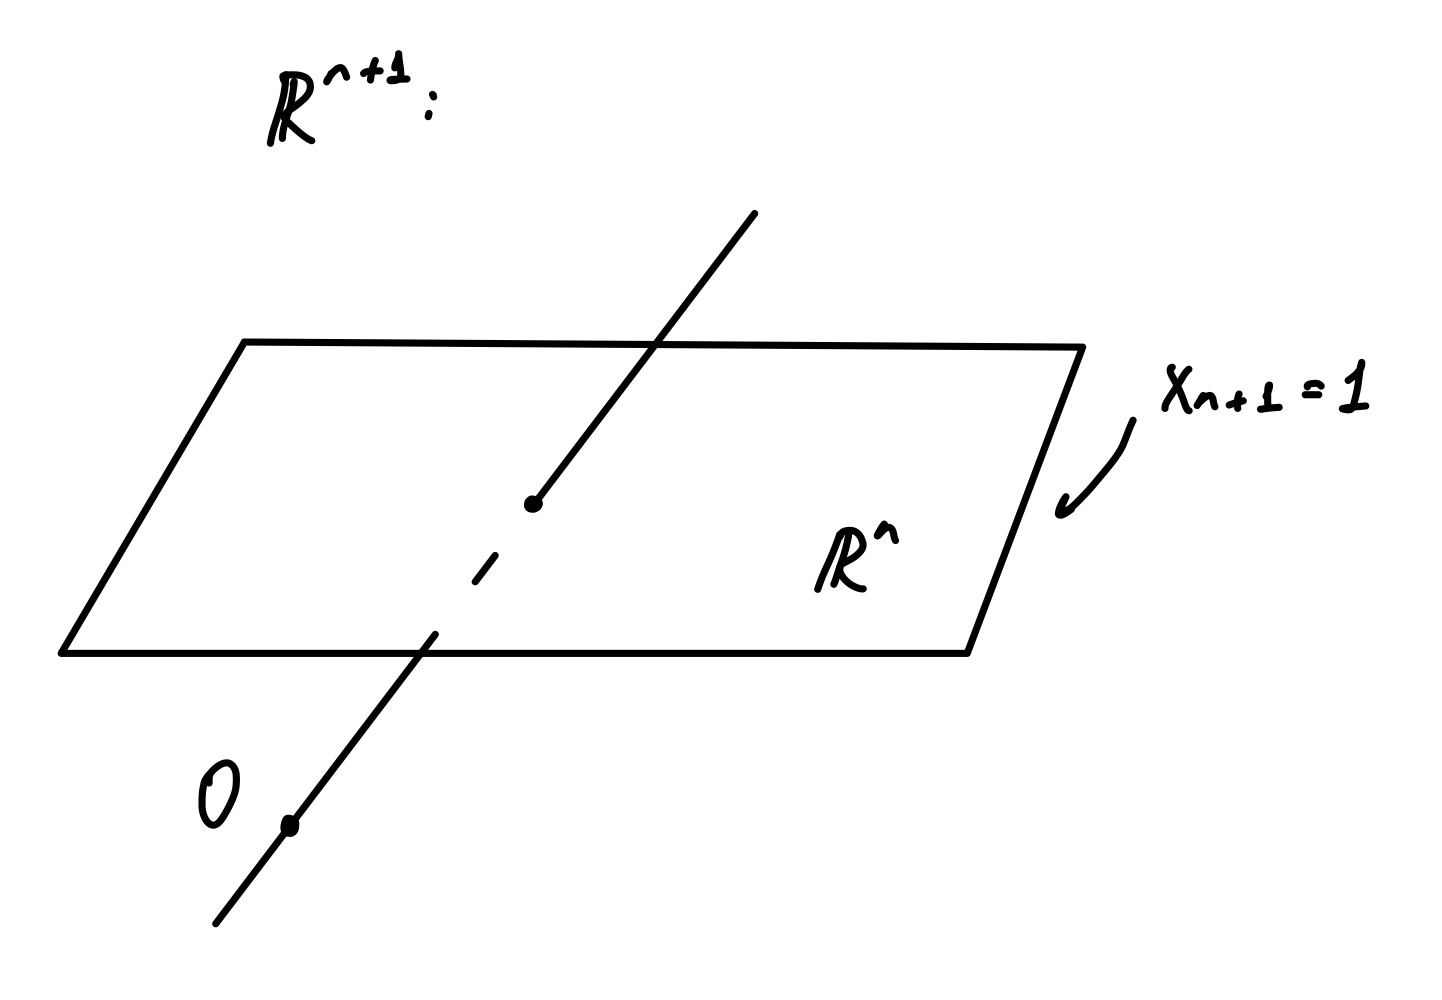
\includegraphics[scale = 0.15]{pic_7.jpeg}
        \caption{Вложение $\mathbb{R}^n$, как плоскости}
    \end{figure}
    \end{center}
    Теперь остается только сказать, что точки, у которых координаты отличаются умножением на константу~--- одна и та же точка.\\

    \subsection{Проективные преобразования и проективный базис. Преобразование Мёбиуса.}

    \begin{example}
    $\mathbb{R}P^1$~--- прямая, к которой мы добавили точку на бесконечности, или же все прямые в $\mathbb{R}^2$, проходящие через 0, то есть, окружность.
     Тогда точке с однородными координатами $[x:y]$ будет соответствовать какой-то прямой, проходящей через точку $(x, y)$, то есть прямой с наклоном $x / y$ и ей будет отвечать $\frac{x}{y} \in \mathbb{R}$, если $y \neq 0$.
    Это так, потому что наше вложение устроено так, что $x \to [x : 1] \sim [ax : a]$. Тогда ясно, что если $y = 0$, то $\forall a, b \ [a, 0] \sim [b, 0]$ и мы отображались из точки бесконечность (которая единственная).
    \end{example}
     \begin{definition}
         Пусть $F\colon \mathbb{P}(V) \to \mathbb{P}(W)$~--- проективное отображение, если оно является проективизацией некоторого линейного отобажения $L\colon V \to W$.
    \end{definition}
    \begin{lemma}
        Пусть $V, W$~--- векторные пространства, а $L\colon V \to W$~---   инъективное линейное отображение. Тогда существует единственное $F\colon \mathbb{P}(V) \to \mathbb{P}(W)$ такое, что
        $p_W \circ L = F \circ p_V$, $p_W \colon W \setminus \{ 0\} \to \mathbb{P}(W)$, $p_V \colon V \setminus \{ 0\} \to \mathbb{P}(V)$.
        Иными словами, коммутативна диаграмма:
        \begin{center}
            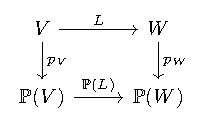
\includegraphics[scale = 1.2]{cd_2.pdf}
        \end{center}
    \end{lemma}
    \begin{proof}
        $L$ переводит прямые через 0 в прямые через 0 (так как это линейное отображение между векторными пространствами), а прямым через 0 отвечают как раз точки $\mathbb{P}(V)$.
    \end{proof}
    \begin{example}
        $ \mathbb{R}P^1 = \widehat{\mathbb{R}} = \mathbb{R} \cup \{ \infty \}$, $x \to [x : 1], \ [x : y] \to \frac{x}{y}$, если $y \neq 0$ и в $\infty$, если $y = 0$.
        Так как $\mathbb{R}P^1$~--- это все прямые в $\mathbb{R}^2$, проективное преобразование проективной прямой на себя~--- проективизация линейного отображения из $\mathbb{R}^2$ на себя. Ясно, что линейное отображение устроено вот так:
        \[ (x,  y) \to (ax + by , cx + dy), \ a, b, c, d \in \mathbb{R}, \ ad - bc \neq 0 \]
        Когда мы рассматриваем проективизацию, нам важно только, на какой прямой лежит образ, то есть
        \[ [x,  y] \to [ax + by , cx + dy], \ a, b, c, d \in \mathbb{R}, \ ad - bc \neq 0 \]
        (Важно, что линейное отображение инъективно, поэтому там везде сказано, что определитель не равен 0).\\
        Возвращаясь обратно к координатам в $\widehat{\mathbb{R}}$ мы получаем, что это $x \to (ax + b / cx + d)$, так как $[x : 1] \to [ax + b, cx + d] = [(ax + b) / (cx + d) : 1]$, если $cx + d \neq 0$. Если же $cx + d = 0$, то ясно, что мы перешли в точку $\infty$. Если же $x = \infty$, то ясно, что $[1 : 0] \to [a : c] = [a / c : 1] \ (c \neq 0)$ (если $c = 0$, то $[1 : 0] \to [1 : 0]$, то бишь $\infty \to \infty$, так как у нас просто линейное отображение $(a /d)x + (b / d)$).\\
        То есть, дробно линейное преобразование на $\mathbb{R}$~--- проективное преобразование. Также теперь ясно, что дробно-линейные преобразования на $\mathbb{R}P^1$ образуют группу (так как они теперь биективны и у нас нет проблем с занулением знаменателя).
    \end{example}

    \begin{example}
    Рассмотрим  биективное на проективной прямой дробно линейное преобразование
        \[ x \to \cfrac{ax + b}{cx + d}\]
        и зададимся вопросом, значения в скольки точках нам нужно знать, чтоб однозначно определить параметры $a, b, c, d$. Засчет того, что в однородных координатах всё происходит с точностью до мультипликативной константы, нам достаточно знать значения всего в трёх точках:
        \[ [0 : 1] \to b / d, \ [1 : 1] \to (a + b) / (c + d), \ [1 : 0] \to a / c\]
        Поскольку нас интересует всё с точностью до пропорциональности, можно считать $d = 1$. Отсюда получаем систему из 3-х уравнений, откуда однозначно находятся все коэффиценты. То есть, для того, чтобы однозначно задать дробно линейное преобразование, нам нужно задать, куда переходят точки $0, 1, \infty$.
    \end{example}

    \begin{definition}[Проективный базис]
        Пусть $X$~--- проективное пространство размерности $n$.  Проективным базисом будем называть набор из  $(n + 2)$-х точек, никакие $(n + 1)$ из которых не лежат в одной  гиперплоскости.
    \end{definition}

    \section{Квадратичные формы и квадрики}
    \subsection{Билинейные формы}

    \begin{definition}[Билинейная форма]
    Пусть $X$~--- векторное пространство. Функция $B: X \times X \to \mathbb{R}$ называется билинейной формой на $X$, если она линейная по каждому аргументу.
    \end{definition}

    \begin{remark}
    Билинейную форму (и не обязательно её, а любую функцию $B: X \times X \to \mathbb{R}$) называют \textbf{симметричной}, если
    \begin{equation*}
        \forall x, y \in X \ B(x, y) = B(y, x)
    \end{equation*}
    \end{remark}

    \begin{remark}
    Подразумевается, что $X$~--- векторное пространство над полем $\mathbb{R}$. Для векторного пространства над другим полем всё определяется аналогично.
    \end{remark}

    \begin{definition}[Матрица билинейной формы]
    Зафиксируем базис $\{v_1, v_2, \hdots, v_n\}$ пространства $X$. В таком случае матрица билинейной формы $B$ на $X$ определяется как матрица $b$ размера $n \times n$, каждый член которой задаётся так:
    \begin{equation*}
        b_{ij} = B(v_i, v_j)
    \end{equation*}
    \end{definition}

    \begin{remark}
    Допустим, нам известна матрица $B_{v}$ билинейной формы $B$ над векторным пространством $X$ в базисе $\{v_1, v_2, \hdots, v_n\}$. В таком случае для точек $x = (x_1, \hdots, x_n)$ и $y = (y_1, \hdots, y_n)$ значение билинейной формы будет следующим:
    \begin{equation*}
        B(x, y) = \sum_{i, j = 1}^{n} [B_{v}]_{ij} x_i y_j
    \end{equation*}
    Что в матричной форме записывается как
    \begin{equation*}
        B(x, y) = x^{T} b y
    \end{equation*}
    \end{remark}

    \begin{remark}
    При фиксированном базисе пространства $X$ существует взаимно однозначное соответствие между матрицами $n \times n$ и билинейными формами, что им соответствуют. При таком сопоставлении симметричным матрицам соответствуют симметричных билинейные формы, и наоборот.
    \end{remark}

    \vspace{15pt}

    Зафиксируем векторное пространство $X$, его базис $v = \{v_1, \hdots, v_n\}$, какой-то ещё его базис $w = \{w_1, \hdots, w_n\}$, билинейную форму на $X$~--- обозначим её $B$. Обозначим $B_u$~--- матрицу $B$ при базисе $u$. Тогда
    \begin{equation*}
        B_v = A^{T} B_w A
    \end{equation*}
    где $A$~--- матрица перехода от $v$ к $w$.

    \begin{proof}
    В самом деле, рассмотрим билинейную форму на базисных векторах $w_i$ и $w_j$, воспользовавшись матрицей в базисе $v$. Тогда
    \begin{equation*}
        w_i^{T} B_w w_j = v_{i}^{T} A^T B_w A v_j = v_{i}^{T} B_v v_{j}
    \end{equation*}
    \end{proof}

    \newpage

    \subsection{Квадратичные формы}

    \begin{definition}[Квадратичная форма]
    Пусть $X$~--- векторное пространство, $Q: X \to \mathbb{R}$. Тогда $Q$ называется квадратичной формой, если существует билинейная форма $B$ на $X$, такая что
    \begin{equation*}
        \forall x \in X \ Q(x) = B(x, x)
    \end{equation*}
    \end{definition}

    \begin{theorem}[О единственной симметричной форме]
    Для любой квадратичной формы $Q$ над векторным пространством $X$ существует единственная симметричная билинейная форма $B$ над тем же пространством, для которой
    \begin{equation*}
        \forall x \in X \ Q(x) = B(x, x)
    \end{equation*}
    \end{theorem}

    \begin{proof}
    Докажем отдельно существование и единственность.
    \begin{itemize}
        \item \textbf{Существование}. По определению существует какая-то билинейная форма $B$, такая что $Q(x) = B(x, x)$. В таком случае, положим форму $C$ так:
        \begin{equation*}
            C(x, y) = \dfrac{B(x, y) + B(y, x)}{2}
        \end{equation*}
        С одной стороны, $C$~--- симметричная и билинейная. С другой стороны~--- $C(x, x) = Q(x)$ для любого $x \in X$.
        \item \textbf{Единственность}. Пусть $Q(x) = B(x, x)$ для некоторой билинейной симметричной формы $B$. Тогда покажем, что $Q$ однозначно определяет все значения $B$:
        \begin{equation*}
            B(x, y) =\dfrac{1}{2}\big((B(x, x) + 2B(x, y) + B(y, y)) - B(x, x) - B(y, y)\big) = \dfrac{1}{2}(Q(x + y) - Q(x) - Q(y))
        \end{equation*}
    \end{itemize}
    \end{proof}

    \begin{remark}
    Это соответствие каноническое, то есть не зависит от выбора базиса пространства $X$.
    \end{remark}

    \begin{remark}
    Таким образом получается биекция между квадратичными формами и билинейными симметричными; при выборе базиса, как уже говорилось, билинейные симметричные формы биективно соответствуют симметричным матрицам подходящего размера. Матрица билинейной симметричной формы $B$ в базисе $v$, соответствующей квадратичной форме $Q$, называется \textbf{матрицей квадратичной формы} $Q$ в базисе $v$.
    \end{remark}

    \begin{corollary}
    Пусть зафиксирован базис $v = \{v_1, v_2, \hdots, v_n\}$ векторного пространства $X$, а также квадратичная форма $Q$ на нём, которой соответствует билинейная симметричная форма $B$ с матрицей $b$ в базисе $v$. Тогда для вектора $x = (x_1, x_2, \hdots, x_n)$ значение квадратичной формы $Q$ находится следующим образом:
    \begin{equation*}
        Q(x) = B(x, x) = \sum_{i, j = 1}^{n} b_{ij} x_i x_j
    \end{equation*}
    \end{corollary}

    \begin{example}[Квадратичная форма в $\mathbb{R}^2$]
    Рассмотрим симметричную матрицу в $\mathbb{R}^2$:
    \begin{equation*}
        \begin{pmatrix}
        a & b\\
        b & c
        \end{pmatrix}
    \end{equation*}
    Тогда квадратичная форма, задаваемая этой матрицей, имеет вид
    \begin{equation*}
        Q\big((x, y)\big) = ax^2 + 2bxy + cy^2
    \end{equation*}
    для любого $(x, y) \in \mathbb{R}^2$.
    \end{example}

    \begin{remark}
    Квадратичная форма (над любым $X$) отождествляется с однородным многочленам степени $2$; это напрямую следует из последнего следствия. \\
    Так как $0$~--- тоже квадратичная форма, то иногда принято считать, что степень $0$ как многочлена равна $2$.
    \end{remark}

    \subsection{Диагонализация билинейных форм}

    В этом параграфе пространство $X$ будем считать снабжённым евклидовой структурой.

    \begin{theorem}[О существовании диагональной матрицы для $Q$]
    Для любой симметричной билинейной формы существует ортонормированный базис, в котором её матрица диагональна.
    \end{theorem}

    \begin{proof}
    Будем доказывать индукцией по размерности пространства. База~--- очевидна, проделаем шаг. Итак, пусть $B$~--- симметричная билинейная форма. Найдём по следующей лемме $v$ такой, что выполнены следующие два условия:
    \begin{itemize}
        \item $|v| = 1$
        \item $\forall w \in v^{\bot} \ B(v, w) = 0$
    \end{itemize}
    Диагонализуем $B|_{W}$, где $W = v^{\bot}$. Базис $\{w_1, w_2, \hdots, w_{n-1}\}$ подпространства $W$ дополняется до базиса пространства $X$ элементом $v$, так как $\forall 1 \leq i \leq n - 1 \ \langle v, w_{i} \rangle = 0$. С другой стороны, так как $\forall 1 \leq i \leq n - 1 \ B(v, w_{i}) = 0$, то матрица $B$ в базисе $\{v, w_1, w_2, \hdots, w_{n-1}\}$ будет иметь нули на всех элементах первой строки и столбца, кроме разве что диагонального, соответствующего $B(v, v)$. Так как $B|_{W}$ мы заранее диагонализовали, то и сама $B$ будет диагональна.
    \end{proof}

    \begin{lemma}
    Для симметричной билинейной формы $B$ на пространстве $X$ размерности $n$ существует вектор $v \in X$ такой, что выполнены следующие два условия:
    \begin{itemize}
        \item $|v| = 1$
        \item $\forall w \in v^{\bot} \ B(v, w) = 0$
    \end{itemize}
    \end{lemma}

    \begin{proof}
    Рассмотрим единичную сферу
    \begin{equation*}
        S^{n - 1} =  \{x \in X \ :\ |x| = 1\}
    \end{equation*}
    Так как $B(x, x)$~--- квадратичная функция, то она непрерывна и достигает максимума на $S^{n - 1}$; скажем, что этот максимум достигается на векторе $v$. \\
    Рассмотрим теперь любой $w$ такой, что $\langle v, w \rangle = 0$ и $|w| = 1$. Натянем плоскость на $v$ и $w$, назовём её $L$. Пересечение $L \cap S^{n - 1}$ есть окружность, а именно
    \begin{equation*}
        \cos(t)v + \sin(t)w
    \end{equation*}
    Найдём $B(\cos(t)v + \sin(t)w, \cos(t)v + \sin(t)w)$:
    \begin{equation*}
        B(\cos(t)v + \sin(t)w, \cos(t)v + \sin(t)w) = \cos(t)^2B(v, v) + \sin(t)^2B(w, w) + 2\cos(t)\sin(t)B(v, w)
    \end{equation*}
    Экстремум (максимум) $B|_L$ будет в точке $t = 0$. Возьмём производную по $t$:
    \begin{equation*}
        B'(\cos(t)v + \sin(t)w, \cos(t)v + \sin(t)w) = -2\cos(t)\sin(t)B(v, v) + 2\cos(t)\sin(t)B(w, w) -
    \end{equation*}
    \begin{equation*}
         - 2\sin^2(t)B(v, w) + 2\cos(t)^2B(v, w)
    \end{equation*}
    Что при $t = 0$ будет равно $2B(v, w)$; с другой стороны, так как экстремум этой непрерывной функции в точке $t = 0$, то в точке $t - 0$ она должна быть равна $0$. Таким образом, получаем $B(v, w) = 0$, а следовательно и $B(v, \alpha w) = 0$ для любого $\alpha$.
    \end{proof}

    \begin{remark}
    Рассмотрим билинейную симметричную форму $B(x, y)$ вида
    \begin{equation*}
        ax^2 + by^2
    \end{equation*}
    при $a > b$. Тогда на единичной сфере
    \begin{equation*}
        S^1 = \{|(x, y)| = 1\}
    \end{equation*}
    максимум $B$ будет равен $a$, тогда как минимум~--- равен $b$:
    \begin{equation*}
        \max_{(x, y) \in S^1} Q(x, y) = a \hspace{20pt} \min_{(x, y) \in S^1} Q(x, y) = b
    \end{equation*}
    \end{remark}

    \begin{remark}
    Понятно, что при диагональной матрице билинейная симметричная форма~--- она же квадратичная форма~--- будет равна
    \begin{equation*}
        Q(x) = a_1x_1^2 + a_2x_2^2 + \hdots + a_nx_n^2
    \end{equation*}
    \end{remark}

    \begin{remark}
    Если не требовать ортонормированности, то сведение к диагональному виду очевидно. К примеру, рассмотрим квадратичную форму $Q$ произвольного вида:
    \begin{equation*}
        Q(x) = a_{11}x_1^2 + a_{12}x_1x_2 + a_{13}x_1x_3 + \hdots + c
    \end{equation*}
    Тогда по индукции заменим $x_i^2$, начиная с $i = 1$ и до $i = n$, следующим образом:
    \begin{equation*}
        (x'_{1})^2 = (a_{11}x_1^2 + \dfrac{a_{12}}{2}x_1x_2 + \dfrac{a_{13}}{2}x_1x_3 + \hdots + \dfrac{a_{1n}}{2}x_1x_n)^2
    \end{equation*}
    После $n$ таких замен мы и получим требуемую форму.
    \end{remark}

    \begin{lemma}
    Числа $a_i$, стоящие на главной диагонали диагональной матрицы квадратичной формы, определены с точностью до перестановки.
    \end{lemma}

    \begin{proof}
    Для квадратичной формы $Q$ существует единственная билинейная симметричная форма $B$, соответствующая ей. Единственный случай, в котором она диагональна~--- это её запись в ортонормированном базисе. Тогда утверждение напрямую следует из того, что собственные числа оператора $B$ не зависят от базиса, а их количество в диагонали матрицы определяется алгебраической кратностью этих чисел в характеристическом многочлене и размерностями соответствующих корневых подпространств.
    \end{proof}

    \subsection{Квадрики на прямой. Проективизация квадрики.}
    В этом параграфе $X = \mathbb{R}$, $F(x) = ax^2 + bx + c$.

    Тогда квадрикой является:
    \begin{itemize}
        \item Любая пара точек
        \item Одна точка (``удвоенная'', в некотором смысле)
        \item Пустое множество
    \end{itemize}

    Рассмотрим проективизацию прямой $\mathbb{R}$, то есть $ \mathbb{R}P^1$, с естественным отображением $x \mapsto [x:1]$ ($\infty = [1:0]$). В таком случае \emph{гомогенизированное уравнение} приобретает вид:
    \begin{equation*}
        F'([x:y]) = ax^2 + bxy + cy^2
    \end{equation*}
    А квадрикой будет множество
    \begin{equation*}
        Q = \{F([x : y] = 0 \ |\ [x:y] \in \mathbb{R}P^1)\}
    \end{equation*}
    удовлетворяющее свойствам
    \begin{itemize}
        \item $[x:y] \in Q \Longleftrightarrow [\lambda x:\lambda y] \in Q$
        \item $Q$ совпадает с $F(x) = 0$ на аффинной карте (при $y = 1$)
    \end{itemize}
    Тем самым из квадрики на прямой можно сделать квадрику на вещественной проективной прямой.

    \begin{remark}
    Если рассматривать гомогенизацию на $\mathbb{C}P^1$, то у всякой квадрики будет ровно две точки.
    \end{remark}

    \begin{remark}
    Аналогично можно гомогенизировать до однородного любой многочлен (не обязательно от одной) переменной.
    \end{remark}

    \subsection{Квадрики на плоскости. Проективные коники, топологическое строение коник на проективной плоскости. }

    \begin{definition}
    Рассмотрим евклидову плоскость $\mathbb{R}^2$ и две фиксированные точки на ней, $X_0$ и $X_1$. Тогда для константы $c \in \mathbb{R}_{>0}$ геометрическое место точек $Y \in \mathbb{R}^2$, таких что $|X_0Y| + |YX_1| = c$, назовём эллипсом $\epsilon$. Иными словами,
    \begin{equation*}
        \epsilon = \{Y \in \mathbb{R}^2 \ :\ |X_0Y| + |YX_1| = c\}
    \end{equation*}
    \end{definition}

    \begin{remark}
    Точки $X_0$ и $X_1$ называют \emph{фокусами} эллипса $\epsilon$.
    \end{remark}

    \begin{lemma}
    \textbf{Принадлежность эллипса к квадрикам}.\\ Всякий эллипс является квадрикой.
    \end{lemma}

    \begin{proof}
    Движением можно переместить фокусы так, чтобы для некоторого положительного $a$:
    \begin{equation*}
        X_0 = (a, 0), \hspace{15pt} X_1 = (-a, 0)
    \end{equation*}
    Тогда исходное условие можно переписать так:
    \begin{equation*}
        \sqrt{(x - a)^2 + y^2} + \sqrt{(x + a)^2 + y^2} = c
    \end{equation*}
    Откуда следует
    \begin{equation*}
        x^2 + 2ax + a^2 + y^2 = c^2 + x^2 -2ax + a^2 + y^2 - 2c\sqrt{(x - a)^2 + y^2}
    \end{equation*}
    То есть
    \begin{equation*}
        2c\sqrt{(x - a)^2 + y^2} = c^2 - 4ax
    \end{equation*}
    Что, в свою очередь, при возведении в квадрат даёт
    \begin{equation*}
        4c^2x^2 - 8ac^2x + 4c^2a^2 + 4c^2y^2 = c^4 - 8axc^2 + 16a^2x^2
    \end{equation*}
    И приведём это к равносильной форме
    \begin{equation*}
        (4c^2 - 16a^2)x^2 + (4c^2)y^2 + (4c^2a^2 - c^4) = 0
    \end{equation*}
    \end{proof}

    \begin{remark}
    Для непустого эллипса мы должны требовать, чтобы $c$ было больше $2a$, иначе эллипс пуст по неравенству треугольника.
    \end{remark}

    \begin{remark}
    Таким образом мы заодно доказали, что эллипс может быть приведён к квадратичной функции без линейных членов. Для непустого эллипса мы может переписать последнее уравнение так, сделав замену:
    \begin{equation*}
        \dfrac{x^2}{A} + \dfrac{y^2}{B} = 1
    \end{equation*}
    Это будет ``каноническим'' уравнением эллипса, из которого очевидно, что с точки зрения аффинной геометрии эллипс ничем не отличается от окружности.
    \end{remark}

    \vspace{10pt}

    Рассмотрим гомогенизацию канонического уравнения эллипса при стандартном вложении $\mathbb{R}^2 \subseteq \mathbb{R}P^2$, $(x, y) \to [x:y:1]$):
    \begin{equation*}
        \dfrac{x^2}{A^2} + \dfrac{y^2}{B^2} = z^2
    \end{equation*}
    Что после аффинного преобразования сводится к уравнению
    \begin{equation*}
        x^2 + y^2 = z^2
    \end{equation*}
    В таком случае в $\mathbb{C}P^2$ эллипсу будут принадлежать точки $[1:i:0]$ и $[1:-i:0]$ в любом случае, что иллюстрирует инвариантность нулей такого многочлена с вещественными коэффициентами при автоморфизмах поля комплексных чисел. \\
    Аналогично, в общем случае можно рассматривать любые полиномиальные функции на аффинных пространствах, а также их гомогенизации и нули этих гомогенизаций.

    \begin{definition}
    Рассмотрим евклидову плоскость $\mathbb{R}^2$ и две фиксированные точки на ней, $X_0$ и $X_1$. Тогда для константы $c \in \mathbb{R}$ геометрическое место точек $Y \in \mathbb{R}^2$, таких что $|X_0Y| - |YX_1| = c$, назовём гиперболой $\gamma$. Иными словами,
    \begin{equation*}
        \gamma = \{Y \in \mathbb{R}^2 \ :\ |X_0Y| - |YX_1| = c\}
    \end{equation*}
    \end{definition}

    \begin{remark}
    Аналогично эллипсу, точки $X_0$ и $X_1$ называют фокусами гиперболы.
    \end{remark}

    \begin{lemma}
    \textbf{Принадлежность гиперболы к квадрикам}.\\ Всякая гипербола является квадрикой.
    \end{lemma}

    \begin{proof}
    Движениями можно переместить фокусы параболы в точки с координатами ($-a$, $0$) и $(a, 0)$ для некоторого положительного $a$. Кроме того, не умаляя общности положим $c \geq 0$, ведь иначе можно просто поменять фокусы местами. Тогда исходное условие можно переписать следующим образом:
    \begin{equation*}
        \sqrt{(x + a)^2 + y^2} - \sqrt{(x - a)^2 + y^2} = c
    \end{equation*}
    С помощью перенесения второго слагаемого направо и возведения в квадрат получим:
    \begin{equation*}
        x^2 + 2ax + a^2 + y^2 = c^2 + 2c\sqrt{(x - a)^2 + y^2} + x^2 - 2ax + a^2 + y^2
    \end{equation*}
    Что равносильно
    \begin{equation*}
        4ax - c^2 = 2c\sqrt{(x - a)^2 + y^2}
    \end{equation*}
    Возведём в квадрат обе части уравнения:
    \begin{equation*}
        16a^2x^2 -8axc^2 + c^4 = 4c^2x^2 - 8axc^2 + 4c^2a^2 + 4c^2y^2
    \end{equation*}
    Преобразуем после сокращения $-8axc^2$:
    \begin{equation*}
        (16a^2 - 4c^2)x^2 - 4c^2y^2 = (4c^2a^2 - c^4)
    \end{equation*}
    \end{proof}

    \begin{remark}
        Для непустой гиперболы нам нужно гарантировать, чтобы $c \leq 2a$ (максимум функции разницы расстояний).
    \end{remark}

    \begin{remark}
    Оценим наши коэффициенты: так как $c \leq 2a$, то $4\cdot(c)^2 \leq 4\cdot(2a)^2$, откуда коэффициент перед $x$ положительный; $4c^2$ положительный по очевидным причинам, последний коэффициент получается из первого умножением на $\dfrac{c^2}{4}$, так что тоже положительный. Значит, поделив на него и заменив буквы, получим
    \begin{equation*}
        \dfrac{x^2}{A^2} - \dfrac{y^2}{B^2} = 1
    \end{equation*}
    то есть каноническое уравнение гиперболы. После аффинного преобразования и гомогенизации получаем:
    \begin{equation*}
        x^2 - y^2 = z^2
    \end{equation*}
    \end{remark}
    \begin{definition}
    Рассмотрим точку $p$ и прямую $l$ в вещественной евклидовой плоскости $\mathbb{R}^2$. Геометрическое место точек, равноудалённых от $p$ и $l$, назовём параболой.
    \end{definition}

    С помощью аффинного преобразования можно положить $p = (0, 1)$, а прямую $\ell\colon y = -1$. В таком случае условие равноудалённости точки $(x, y)$ можно переписать так:

    \begin{equation*}
        \sqrt{x^2 + (y - 1)^2} = \sqrt{(y + 1)^2}
    \end{equation*}

    Что при возведении в квадрат даёт:

    \begin{equation*}
        x^2 - 4y = 0 \Longrightarrow y = \dfrac{x^2}{4}
    \end{equation*}

    Заменой $y \to \dfrac{y}{4}$ (аффинным преобразованием) получаем каноническое уравнение параболы, подтверждающее её принадлежность к квадрикам:

    \begin{equation*}
        y = x^2
    \end{equation*}

    Рассмотрим гомогенизацию параболы в $\mathbb{R}P^2$:

    \begin{equation*}
        yz = x^2
    \end{equation*}

    В таком случае множеству точек, удовлетворяющих данному равенству, принадлежит в том числе и точка $[0:1:0]$~--- бесконечно удалённая точка. Тем самым, ветки параболы в $\mathbb{R}P^2$ ``замыкаются'', а следовательно топологически она ничем не отличается от окружности. Заметим, что гипербола тоже будет окружностью (топологически) в $\mathbb{R}P^2$, но она будет пересекать бесконечно удалённую прямую уже в двух точках. Таким образом получается, что топологически эллипс, парабола и гипербола отличаются только лишь количеством точек пересечения с бесконечно удалённой прямой~--- их 0, 1 и 2 соответственно, что значит их проективные аналоги неотличимы друг от друга.


    Возьмём прямую в $\mathbb{R}^3$ с котангенсом угла наклона $a$. Вращением её относительно оси $Oz$ получим \textbf{конус}, уравнение которого будет
    \begin{equation*}
        z^2 = a^2(x^2 + y^2)
    \end{equation*}

    Заметим, что все встречавшиеся нам квадрики являются сечениями конуса плоскостью, не проходящей через (0, 0, 0):
    \begin{itemize}
        \item Сечением плоскости, перпендикулярной $Oz$, мы получаем окружность.
        \item Постепенно ``наклоняя'' эту плоскость, поворачивая её относительно прямой, лежащей в этой плоскости и параллельной оси $Oy$, мы будем получать эллипсы.
        \item Когда угол наклона будет совпадать с наклоном образующей прямой, мы получим параболу.
        \item Когда угол наклона станет больше, мы получим гиперболу сечением ``верхней'' и ``нижней'' частей конуса.
    \end{itemize}
    \subsection{Проективные квадрики}
    \begin{definition}
        Пусть $Q$~--- квадратичная форма на $\mathbb{R}^{n + 1}$. Тогда ясно, что, так как $Q$~--- однородный многочлен от координат степени 2,
        \[ Q(\lambda x_0, \lambda x_1, \ldots, \lambda x_n) = \lambda^2 Q(x_0, x_1, \ldots, x_n) \]
        Квадрикой в $\mathbb{R}P^n$ называют множество точек, удовлетворяющих однородному уравнению
        \[Q(x_0, x_1, \ldots, x_n) = 0 \]
    \end{definition}
    Рассмотрим сначала вещественные проективные квадрики. Как мы уже поняли, квадратичная форма в  $\mathbb{R}^3$ задаёт
    проективную квадрику.
    Если квадратичная форма невырожденная, то заменой координат её можно привести к одному из четырех видов:
    \begin{itemize}
        \item $x^2 + y^2 + z^2$

        \item $x^2 + y^2 - z^2$

        \item $-x^2 - y^2 + z^2$

        \item $-x^2 - y^2 - z^2$
    \end{itemize}
    Отсюда получаем следующие проективные квадрики:
    \begin{itemize}
        \item $x^2 + y^2 + z^2 = 0$~--- пустое множество.

        \item $x^2 + y^2 - z^2$~--- конус.

        \item $-x^2 - y^2 + z^2$~--- конус.

        \item $-x^2 - y^2 - z^2$~--- пустое множество.
    \end{itemize}
    То есть, все непустые невырожденные квадрики проективно эквивалентны (одна переводится в другую проективной заменой координат).
    Заметим, что рассматривая сечения этого конуса плоскостью (то есть, рассматриваю проективные квадрики в аффинной карте) мы будем получать
    знакомые нам конические сечения, то есть, квадрики на плоскости.
    Теперь рассмотрим комплексные проективные квадрики:

    \subsection{Классификация кривых и поверхностей второго порядка}

    В этом параграфе $X$~--- аффинное пространство, снабжённое евклидовой структурой.

    \begin{theorem}[Декартовы координаты квадратичной функции]
    Пусть $F: X \to \mathbb{R}$~--- квадратичная функция. Тогда существует \textbf{декартова система координат} (точка отсчёта и ортонормированный базис), такой что найдутся $a_1, a_2, \hdots,$  $a_n, b, c \in \mathbb{R}, b > 0$, при которых для любого вектора $x = (x_1, x_2, \hdots, x_n)$ выполняется
    \begin{equation*}
        \left[
      \begin{gathered}
          \begin{gathered}
            F(x) = a_1x_1^2 + a_2x_2^2 + a_3x_3^2 + \hdots + a_nx_n^2 + c
            \\
          \end{gathered}
        \\
          \begin{gathered}
            F(x) = a_1x_1^2 + a_2x_2^2 + \hdots + a_{n-1}x_{n-1}^2 + bx_n
            \\
          \end{gathered}
        \\
      \end{gathered}
    \right.
    \end{equation*}
    то есть функция $F$ имеет одну из этих двух форм в этой системе координат.\end{theorem}


    \begin{proof}
    Разложим функция $F = Q(x) + L(x) + C$, где $Q$~--- квадратичная форма, $L$~--- линейная форма, $C$~--- константа. В какой-то системе координат мы можем добиться, согласно предыдущей теореме,
    \begin{equation*}
    \begin{cases}
        Q(x) = a_1x_1^2 + a_2x_2^2 + \hdots + a_nx_n^2\\
        L(x) = b_1x_1 + b_2x_2 + \hdots b_nx_n
    \end{cases}
    \end{equation*}
    Сделаем это так: для каждого $i$ такого, что $a_i$ и $b_i$ не $0$, будем сдвигать $0$:
    \begin{equation*}
        0 \to -\dfrac{b_i}{2a_i}v_i
    \end{equation*}
    Что соответствует группировке
    \begin{equation*}
        a_ix_i^2 + b_ix_i = a_i(x_i + \dfrac{b_i}{2a_i})^2 + \text{const}
    \end{equation*}
    и замене
    \begin{equation*}
        x_i \to x_i + \dfrac{b_i}{2a_i}
    \end{equation*}
    Таким образом, мы сможем привести функцию $F$ в следующему виду (после перенумерации слагаемых):
    \begin{equation*}
        F(x) = a_1x_1^2 + a_2x_2^2 + \hdots + a_kx_k^2 + b_{k + 1}x_{k + 1} + b_{k + 2}x_{k + 2} + \hdots + b_nx_n + c
    \end{equation*}
    Возьмём базис $(v_1, v_2, \hdots, v_k, v_n$, где $v_1, v_2, \hdots, v_k$~--- старые вектора, а $v_n$ определяется как
    \begin{equation*}
        v_n = \dfrac{b_{k + 1}v_{k+1} + b_{k + 2}v_{k + 2} + \hdots + b_{n - 1}v_{n - 1} + b_{n}x_n}{\sqrt{b_{k+1}^2 + b_{k+2}^2 + \hdots + b_{n}^2}}
    \end{equation*}
    В таком базисе, обозначив
    \begin{equation*}
        b = \sqrt{b_{k+1}^2 + b_{k+2}^2 + \hdots + b_{n}^2} > 0
    \end{equation*}
    Функция $F$ принимает вид
    \begin{equation*}
        F(x) = a_1x_1^2 + a_2x_2^2 + \hdots + a_kx_k^2 + bx_n + c
    \end{equation*}
    и перенесём начало на $-\dfrac{c}{b_n}v_n$. Если $b$ стало меньше $0$, то заменой $x_n \to -x_n$ оно станет вновь положительным. Таким образом, у нас возможны две ситуации, при $b > 0$ и при $b = 0$. Оба этих случая и приводят нас к соответствующему ответу.
    \end{proof}

    \begin{theorem}\textbf{(Классификация квадрик в $\mathbb{R}^2$)}\\
    Любая квадрика на плоскости $\mathbb{R}^2$ есть один из следующих видов:
    \begin{itemize}
        \item Пустое множество: например, $x^2 + y^2 + 1 = 0$.
        \item Точка: например, $x^2 + y^2 = 0$.
        \item Прямая: например, $x^2 = 0$.
        \item Две параллельные прямые: например, $(ax + by + c)(a'x + b'y + c') = 0$.
        \item Две пересекающиеся прямые: например, $(ax + by + c)(a'x + b'y + c') = 0$.
        \item Парабола: аффинно она связна, неограничена и не содержит прямых.
        \item Эллипс: аффинно он ограничен и не содержит прямых.
        \item Гипербола: аффинно она не связна, неограничена и не содержит прямых.
    \end{itemize}
    \end{theorem}

    \begin{proof}
    Будем считать, что эти варианты различны, так как в формулировке теоремы обоснованы их различия относительно аффинных преобразований. Согласно теореме о декартовых координатах квадратичной функции, уравнение квадрики можно свети к одному из двух следующих вариантов:
    \begin{equation*}
            \left[
      \begin{gathered}
          \begin{gathered}
            ax^2 + by = 0
            \\
          \end{gathered}
        \\
          \begin{gathered}
            ax^2 + by^2 + c = 0
            \\
          \end{gathered}
        \\
      \end{gathered}
    \right.
    \end{equation*}
    где $a \neq 0$. Итак, рассмотрим все варианты отдельно:
    \begin{enumerate}
        \item Пусть функция свелась к $ax^2 + by = 0$. Тогда возможны два случая:
        \begin{itemize}
            \item Если $b = 0$, то это прямая.
            \item Если $b \neq 0$, то это парабола.
        \end{itemize}
        \item Пусть функция свелась к $ax^2 + by^2 + c = 0$. Не умаляя общности, положим $a > 0$. Рассмотрим случаи:
    \begin{itemize}
        \item Пусть $c = 0$. Если $b > 0$, то мы получаем уравнение точки. Если $b = 0$, то это прямая. Если же $b < 0$, то это две пересекающиеся прямые.
        \item Пусть $c > 0$. Тогда, если $b \geq 0$, то это пустое множество; если же $b < 0$, то мы имеем уравнение гиперболы.
        \item Пусть $c < 0$. Тогда, если $b > 0$, то это эллипс. Если $b < 0$, то это вновь гипербола. Если же $b = 0$, то это две параллельные прямые.
    \end{itemize}
    \end{enumerate}
    \end{proof}
    \subsection{Принцип Минковского-Хассе для квадратичных форм.}

    В этом параграфе мы займемся доказательством одного из самых красивых и геометричных фактов в алгебраической теории чисел.
    Поговорим вначале просто о квадратичных формах на $\mathbb{Q}_p$.\\
    Так как тоерема о диагонализации верна над произвольным полем, а $\mathbb{Q}_p$~--- поле, любая квадратичная форма на $\mathbb{Q}_p$ представима в виде
    \[ F(x) = \alpha_1 x_1^2 + \ldots + \alpha_n x_n^2, \ \alpha_i \neq 0 \]
    причем ясно, что либо $\alpha_i = p^{2k_i} \varepsilon_i$, либо $\alpha_i = p^{2k_i + 1} \varepsilon_i$, где $\varepsilon_i \in \mathbb{Z}_p^{*}$.

    Делая замены вида $y_i = p^{k_i} x_i$ мы всегда сможем привести форму к виду
    \[ F(x) = \varepsilon_1 x_1^2 + \varepsilon_2 x_2^2 + \ldots + \varepsilon_r x_r^2  + p(\varpesilon_{r + 1} x_{r+ 1}^2 + \ldots + \varepsilon_{r + n} x_{r + n}^2) = F_0 + pF_1 \]
    Заметим, что над $\mathbb{Q}_p$ эта форма будет эквивалента форме $F_1 + pF_0$. Для доказательства центральной теоремы этого параграфа нам понадобится следующая лемма:

    \begin{lemma}
        Если $p \enq 2$ и $0 < r < n$, а $F = F_1 + pF_0$, то форма $F$ представляет 0 над $\mathbb{Q}_p$ тогда и только тогда, когда
        $F_0$ или $F_1$ представляет $0$ над $\mathbb{Q}_p$.
    \end{lemma}
    а точнее,её следствие:

    \begin{corollary}\label{MincCor}
        Если $\varepsilon_1, \ldots, \varepsilon_n \in \mathbb{Z}_p^{*}$, то $f = \varepsilon_1 x_1^2 + \ldots + \varepsilon_r x_r^2 $ представляет
        0 над $\mathbb{Q}_p$ тогда и только тогда, когда сравнение
        \[ f(x_1, \ldots, x_r) \equiv 0 \pmod{p} \]
        имеет в $\mathbb{Z}_p$ нетривиальное решение.
     \end{corollary}
    Всё это доказывается достаточно быстро, но, к сожалению, сейчас совершенно нет времени на такие проверки.
    Приступим наконец к доказательству теоремы.
    \begin{theorem} \textbf{(Минковского-Хассе)}\\
        Рациональная квадратичная форма представляет 0 над полем $\mathbb{Q}$ тогда и только тогда, когда она представляет 0 над $\mathbb{R}$
        и над $\mathbb{Q}_p$ для всех простых $p$.
    \end{theorem}
    \begin{proof}
        В доказательстве мы рассмотрим канонически самый важный случай, где $n = 3$. \\
        Сразу отметим, что импликация в одну из сторон очевидна, так как $\mathbb{Q} \hookrightarrow \mathbb{R}$ и $\mathbb{Q} \hookrightarrow \mathbb{Q}_p$.

         И так, по теореме о диагонализации квадратичной формы, наша форма рациональной заменой базиса приводится к виду
        \[ F(x) = a_1 x_1^2 + a_2 x_2^2 + a_3 x_3^2, \quad a_1 a_2 a_3 \neq 0 \]
        Так как она представляет 0 над $\mathbb{R}$, все три коэффицента не могут быть одного знака. Домножая на $-1$ мы всегда сможем
        добиться $a_1, a_2 > 0, \ a_3 < 0$. \\

        Мы можем рассматривать $a_i \in \mathbb{Z}$ (домножив на $\lcm$ знаменателей), свободными от квадратов, так как если
        $a_1 \divisible p^2$ для некоторого $p$ (то есть, $a_1 = p^2 u$), мы всегда можем сделать
        \[  p^2 u \cdot x_1^2 + a_2 x_2^2 + a_3 x_3^2 \to u (x_1 p)^2 + a_2 x_2^2 + a_3 x_3^2 \to a_1' x_1'^2 + a_2 x_2^2 + a_3 x_3^2. \]
        Кроме того, можно полагать их попарно взаимно простыми, так как если $a_1 \divisible p$ и $a_2 \divisible p$, то домножая на $p$  мы имеем
        \[a_1 x_1^2 + a_2 x_2^2 + a_3 x_3^2 \to \frac{a_1}{p}(p x_1)^2 + \frac{a_2}{p} (p x_2) + pa_3 x_3^2 \to a_1' x_1'^2 + a_2' x_2'^2 + a_3' x_3^2\]
        Таким образом, мы свели задачу к рассмотрению формы
        \[ F(x, y, z) = ax^2 + by^2 - cz^2 \]
        где $a, b, c$~--- попарно взаимно простые свободные от квадратов натуральные числа.\\

        Пусть $p$~--- простой делитель $c$ (тогда $a \not\divisible p$, $b \not\divisible p$), а $(x_0, y_0, z_0)$~--- ненулевое решение
        уравнения $F(x, y, z) = 0$ над $\mathbb{Q}_p$.

        По следствию \ref{MincCor} это влечет, что сравнение
        \[ ax^2 + by^2 \equiv 0 \pmod{p} \]
        имеет нетривиальное решение, обозначим его за $(x_0, y_0)$. Тогда ясно, что
        \[ b \equiv y_0^{-2} (-ax_0^2) \pmod{p}\]
        а отсюда мы имеем
        \[ ax^2 + bx^2 \equiv a y_0^{-2} (x y_0 + y x_0)(x y_0 - y x_0) \pmod{p} \]
        аналогичное разложение мы будем иметь и по модулю всех простых $p$, делящих коэффицент $a$ и коэффицент $b$.\\
        Таким образом, для любого простого $p$, делящего $abc$ существуют линейные формы $M^{p}$ и $L^{(p)}$, для которых
        \[ F \equiv L^{(p)} M^{(p)} \pmod{p} \]
        По китайской теореме об остатках найдем такие целочисленные линейные формы $L$ и $M$, что
        \[ L \equiv L^{(p)} \pmod{p}, M \equiv M^{(p)} \pmod{p} \quad \forall p \ \text{~--- простое, } p \mid abc \]
        и соответственно $F \equiv LM \pmod{abc}$. Будем рассматривать целочисленные $x, y, z$ в диапазоне
        \[ 0 \le x < \sqrt{bc}, \ 0 \le y < \sqrt{ac}, \ 0 \le z < \sqrt{ab} \text{~--- } (\ddot\smile) \]
        Если рассматривать случаи, кроме $a, b, c = 1$, то не все числа из тройки $\sqrt{ab}, \sqrt{ac}, \sqrt{bc}$ целые (так как $a, b, c$~--- попарно взаимно простые), а значит,
        число троек $(x, y, z)$, удовлетворяющих $(\ddot\smile)$ больше, чем $\sqrt{ac} \sqrt{ab}\sqrt{bc} = abc$.\\

        Отсюда следует, что существуют две различные тройки, на которых $L$ принимает одно и тоже значение по модулю $abc$, то есть
        \[ L(x_1, y_1, z_1) \equiv m \pmod{abc} , \ L(x_2, y_2, z_2) \equiv m \pmod{abc}.\]
        Так как форма $L$ линейная, это влечет $L(x_1 - x_2, y_1 - y_2, z_1 - z_2) \equiv 0 \pmod{abc}$, то есть мы нашли такие
        $(x_0, y_0, z_0)$, где $|x_0| < \sqrt{bc}, \ |y_0| < \sqrt{ac}, \ |z_0| < \sqrt{ab}$ и $L(x_0, y_0, z_0) \equiv 0 \pmod{abc}$.
        \[ F \equiv L M \pmod{abc} \Rightarrow a x_0^2 + b y_0^2 - c z_0^2 \equiv 0 \pmod{p} , \ -abc < ax_0^2 + by_0^2 - cz_0^2 < 2abc. \]

        Из оценки следует, что либо $a x_{0}^2 + b y_0^2 - cz_0^2 = 0$, $a x_{0}^2 + b y_0^2 - cz_0^2 = abc$. В первом случае теорема доказана, во второ случае
        нужный результат следует из \textcolor{red}{хитрого тождества:}
        \[ a(x_0 z_0 + b y_0)^2 + b(y_0 z_0 - a x_0)^2 - c(z_0 + ab)^2 = 0 \]

    \end{proof}
    \section{Кубические уравнения и эллиптические кривые.}
    \subsection{Существование рациональных решений.}
    Оказывается, что в отличие от квадратичных форм, для рациональных кубических форм $F(x, y, z)$ не существует (пока не найдено)
    алгоритма, который позволяет установить существование нетривиальных рациональных решений уравнения $F = 0$, хотя изучено большое количество конкретных уравнений, например
    \[ ax^3 + by^3 + cz^3 = 0 \]
    Связано это во многом с тем, что для кубических форм перестает выполнятся принцип Минковского-Хассе. Например, уравнение
    \[ 3x^2 + 4y^2 + 5z^2 0 \]
    имеет нетривиальные решения над $\mathbb{R}$ и над $\mathbb{Q}_p$ для всех простых $p$, но не имеет нетривиальных решений над $\mathbb{Q}$.
    \subsection{Эллпитические кривые.}

    \begin{definition}
        Плоской алгебраической кривой называт кривую в $\mathbb{C}P^2$, заданную однородным полиномиальным уравнением
        \[ \sum\limits_{i + j + k} a_{i j k} x^{i} y^{j} z^{k} = 0, \ i, j, k \in \mathbb{Z}_{\ge 0}, \ \exists (i, j, k)\colon a_{i j k} \neq 0 \]

    \end{definition}
\end{document}
